\documentclass[a4paper, 10pt, garamond, oneside]{book}
\usepackage{cours-preambule}

\toggletrue{student}
\HideSolutionstrue

\makeatletter
\renewcommand{\@chapapp}{MPSI3 -- \today\ -- Devoir surveillé}
\makeatother

\graphicspath{{./figures/}{./figures/E1}{./figures/E2}{./figures/P1}{./figures/P2}}

\setlist[enumerate]{resume}
\setlist[enumerate,1]{leftmargin=10pt, label=\sqenumi}
\setlist[enumerate,2]{leftmargin=20pt, label=\Alph*)}

\newcommand{\figsvg}[1]{
  \begin{center}
    \subimport{figures/}{#1}
  \end{center}
}
\newcommand{\figsvgCap}[2]{
  \begin{center}
    \subimport{figures/}{#1}
    \captionof{figure}{#2}
  \end{center}
}

\begin{document}
\setcounter{chapter}{0}
\chapter{Optique géométrique\ifprof{\!\!-- corrigé}}
\label{ch:ds01}

\ifstudent{
\begin{center}
	\Large\bfseries
	\xul{Tout moyen de communication est interdit}
	\smallbreak
	\xul{Les téléphones portables doivent être éteints et rangés dans les sacs}
	\smallbreak
	\xul{Les calculatrices sont \textit{autorisées}}
\end{center}
\begin{prgm}
  \vspace{6pt}
  \begin{tcb}*[cnt, bld, fontupper=\large](ror){}
    Toute l'optique géométrique de MPSI.
  \end{tcb}
  \vspace{-8pt}
\end{prgm}
Le devoir est composé des parties \textit{indépendantes} suivantes~:
{\Large
\begin{itemize}[label=$\diamond$]
	\bitem{Exercice 1}~: Étude de quelques lentilles minces
	\bitem{Exercice 2}~: Instruments d'optiques à l'infini -- deux parties
  indépendantes
	\bitem{Problème 1}~: Étude de pierres précieuses
	\bitem{Problème 2}~: Image au fond d'un gobelet
\end{itemize}
}

Les différentes questions peuvent être traitées dans l'ordre désiré.
\textbf{Cependant}, le numéro complet de la question doit être indiqué, et
\textbf{vous indiquerez si vous traitez la question d'un exercice sur une page
	complètement déconnectée}, sous peine de n'être ni vue ni corrigée.
\bigbreak
Une attention particulière sera portée à la \textbf{qualité de rédaction}. Les
hypothèses doivent être clairement énoncées, les propositions reliées entre
elles par des connecteurs logiques, les lois et théorèmes énoncés, sans pour
autant devenir une composition de français.
\bigbreak
De plus, la \textbf{présentation} de la copie sera prise en compte. Outre la
numérotation des questions, l'écriture, l'orthographe, les encadrements, la
marge, le cadre laissé pour la note et le commentaire font partie des points à
travailler. Il est notamment attendu que \textbf{les expressions littérales
	soient encadrées}, que \textbf{les calculs n'apparaissent pas} mais que le
détail des grandeurs avec leurs unités soit indiqué, et \textbf{les applications
	numériques soulignées}.
\bigbreak
Ainsi, l'étudiant-e s'expose aux malus suivants concernant la forme et le fond~:
\begin{tcb}*(prop)"bomb"{Malus}
	\begin{minipage}{0.50\linewidth}
		\begin{itemize}
			\item A~: application numérique mal faite~;
			\item N~: numéro de copie manquant~;
			\item P~: prénom manquant~;
			\item E~: manque d'encadrement des réponses~;
			\item M~: marge non laissée ou trop grande~;
			\item V~: confusion ou oubli de vecteurs~;
		\end{itemize}
	\end{minipage}
	\begin{minipage}{0.50\linewidth}
		\begin{itemize}
			\item Q~: question mal ou non indiquée (même passées)~;
			\item C~: copie grand carreaux~;
			\item U~: mauvaise unité (flagrante)~;
			\item H~: homogénéité non respectée~;
			\item S~: chiffres significatifs non cohérents~;
			\item $\f$~: loi physique fondamentale brisée.
		\end{itemize}
	\end{minipage}
\end{tcb}

\begin{tcb}(impo){Exemple application numérique}
	\vspace*{-10pt}
	\begin{minipage}{0.45\linewidth}
		\begin{gather*}
			\boxed{n = \frac{PV}{RT}}
			\qav
			\left\{
			\begin{array}{rcl}
				p & = & \SI{1.0e5}{Pa}                \\
				V & = & \SI{1.0e-3}{m^3}              \\
				R & = & \SI{8.314}{J.mol^{-1}.K^{-1}} \\
				T & = & \SI{300}{K}
			\end{array}
			\right.\\
			\mathrm{A.N.~:}\quad
			\xul{n = \SI{5.6e-4}{mol}}
		\end{gather*}
	\end{minipage}
	\hfill
	\cancel{\bcancel{
			\begin{minipage}{0.45\linewidth}
				\begin{gather*}
					n = \frac{PV}{RT} = \frac{\num{e5}\cdot\num{1}}{8.32\cdot300}
					= 0.56
				\end{gather*}
			\end{minipage}
		}}
\end{tcb}
\newpage
}

\exercice[46]{Étude de quelques lentilles minces \ifprof{\hfill \small D'après IESSA 2022 \hfill}}

\subsection{Lentille convergente de focale donnée}

\switch{
	On considère une lentille convergente $\Lc$ de centre optique O et de distance
	focale $f' = \SI{20}{cm}$. Elle est utilisée dans les conditions de
	\textsc{Gauss} sur un banc d'optique. Elle donne d'un objet A sur l'axe
	optique une image A\bp sur l'axe optique.
	\smallbreak
	Pour les trois questions suivantes~:
	\begin{itemize}
		\item Faire un schéma à l'échelle~;
		\item Caractériser l'image (virtuelle ou réelle, droite ou renversée,
		      agrandie, de même taille ou rétrécie)~;
		\item Déterminer par le calcul la position de l'image~;
		\item Calculer le grandissement~.
	\end{itemize}

	\begin{enumerate}
		\item On considère un objet réel AB perpendiculaire à l'axe optique et placé
		      à \SI{40}{cm} de la lentille.
		\item On considère un objet réel AB perpendiculaire à l'axe optique est
		      placé à \SI{10}{cm} de la lentille.
		\item On considère un objet virtuel AB perpendiculaire à l'axe optique est
		      placé à \SI{20}{cm} de la lentille.
	\end{enumerate}
}{
	\begin{enumerate}
		\item
		      \noindent
		      \begin{minipage}[t]{.48\linewidth}
			      On obtient donc une image \xul{réelle}, \xul{renversée} et de
			      \xul{même taille} que l'objet. Avec la relation de
			      \textsc{Descartes}~:
			      \begin{gather*}
				      \frac{1}{f'} =  \frac{1}{\OAp}-\frac{1}{\OA}
				      \\\Lra
				      \frac{1}{\OAp} = \frac{1}{\OA}+\frac{1}{f'}= \frac{\OA+f'}{\OA f'}
				      \\\Lra
				      \boxed{\OAp = \frac{\OA f'}{\OA+f'}}
				      \qav
				      \left\{
				      \begin{array}{rcl}
					      \OA & = & \SI{-40}{cm}
					      \\
					      f'  & = & \SI{20}{cm}
				      \end{array}
				      \right.\\
				      \AN
				      \xul{
					      \OAp = \SI{40}{cm}
				      }
			      \end{gather*}
			      De plus,
			      \begin{gather*}
				      \boxed{\gamma = \frac{\OAp}{\OA}}
				      \qav
				      \left\{
				      \begin{array}{rcl}
					      \OAp & = & \SI{40}{cm}
					      \\
					      \OA  & = & \SI{-20}{cm}
				      \end{array}
				      \right.\\
				      \AN
				      \xul{
					      \gamma = -1
				      }
			      \end{gather*}
		      \end{minipage}
		      \hfill
		      \begin{minipage}[t]{.48\linewidth}
			      ~
			      \begin{center}
				      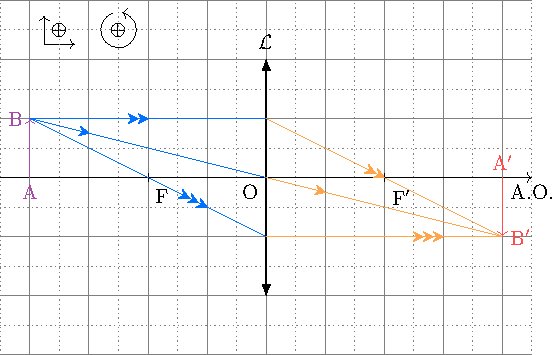
\includegraphics[width=\linewidth]{convAF}
			      \end{center}
		      \end{minipage}
		\item
		      \noindent
		      \begin{minipage}[t]{.48\linewidth}
			      On obtient donc une image \xul{virtuelle}, \xul{droite} et
			      \xul{agrandie}. Avec la relation de \textsc{Descartes}~:
			      \begin{gather*}
				      \boxed{\OAp = \frac{\OA f'}{\OA+f'}}
				      \qav
				      \left\{
				      \begin{array}{rcl}
					      \OA & = & \SI{-10}{cm}
					      \\
					      f'  & = & \SI{20}{cm}
				      \end{array}
				      \right.\\
				      \AN
				      \xul{
					      \OAp = \SI{-20}{cm}
				      }
			      \end{gather*}
			      De plus,
			      \begin{gather*}
				      \boxed{\gamma = \frac{\OAp}{\OA}}
				      \qav
				      \left\{
				      \begin{array}{rcl}
					      \OAp & = & \SI{-20}{cm}
					      \\
					      \OA  & = & \SI{-10}{cm}
				      \end{array}
				      \right.\\
				      \AN
				      \xul{
					      \gamma = +2
				      }
			      \end{gather*}
		      \end{minipage}
		      \hfill
		      \begin{minipage}[t]{.48\linewidth}
			      ~
			      \begin{center}
				      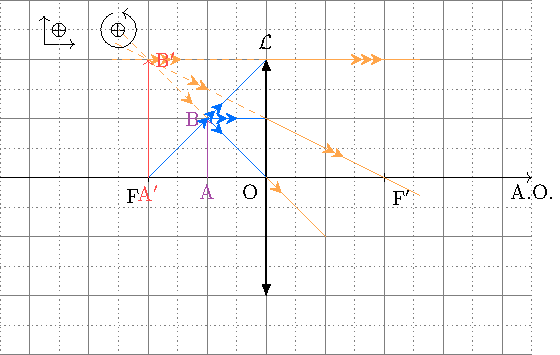
\includegraphics[width=\linewidth]{convCF}
			      \end{center}
		      \end{minipage}
		\item
		      \noindent
		      \begin{minipage}[t]{.48\linewidth}

			      On obtient donc une image \xul{réelle}, \xul{droite} et
			      \xul{rétrécie}. Avec la relation de \textsc{Descartes}~:

			      \begin{gather*}
				      \boxed{\OAp = \frac{\OA f'}{\OA+f'}}
				      \qav
				      \left\{
				      \begin{array}{rcl}
					      \OA & = & \SI{20}{cm}
					      \\
					      f'  & = & \SI{20}{cm}
				      \end{array}
				      \right.\\
				      \AN
				      \xul{
					      \OAp = \SI{10}{cm}
				      }
			      \end{gather*}
			      De plus,
			      \begin{gather*}
				      \boxed{\gamma = \frac{\OAp}{\OA}}
				      \qav
				      \left\{
				      \begin{array}{rcl}
					      \OAp & = & \SI{10}{cm}
					      \\
					      \OA  & = & \SI{20}{cm}
				      \end{array}
				      \right.\\
				      \AN
				      \xul{
					      \gamma = +0.5
				      }
			      \end{gather*}
		      \end{minipage}
		      \hfill
		      \begin{minipage}[t]{.48\linewidth}
			      ~
			      \begin{center}
				      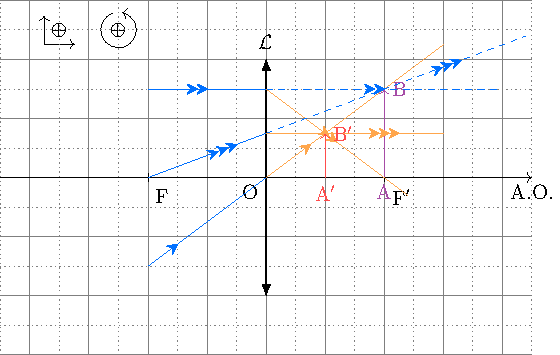
\includegraphics[width=\linewidth]{convDF}
			      \end{center}
		      \end{minipage}
	\end{enumerate}
}

\subsection{Lentille convergente quelconque}
\switch{
	\begin{enumerate}
		\item Dans ce cas, l'image d'un objet réel est-elle toujours réelle~?
		      Toujours virtuelle~? Ou aucune de ces deux affirmations n'est
		      correcte~? Justifier.
		\item L'image d'un objet virtuel est-elle toujours réelle~? Toujours
		      virtuelle~? Ou aucune de ces deux affirmations n'est correcte~?
		      Justifier.
	\end{enumerate}
}{
	\begin{enumerate}
		\item Les questions 1 et 2 montrent que pour un objet réel, une lentille
		      convergente peut donner aussi bien une image réelle (question~1) que
		      virtuelle (question~2). Donc pour l'image d'un objet réel à travers
		      une lentille convergente, les deux cas peuvent se présenter.
		\item Nous avons vu qu'avec la relation de \textsc{Descartes}, en isolant
		      $\OAp$ on obtenait
		      \[
			      \OAp = \frac{\OA f'}{\OA + f'}
		      \]
		      Si l'objet est virtuel, alors $\OA > 0$. Or, la lentille est
		      convergente, donc $f' > 0$. Ainsi, $\OAp > 0$. En conclusion, l'image
		      d'un objet virtuel au travers d'une lentille convergente est
		      \xul{toujours réelle}.
	\end{enumerate}
}

\subsection{Lentille divergente quelconque}
\switch{
	\begin{enumerate}
		\item Dans ce cas, l'image d'un objet réel est-elle toujours réelle~?
		      Toujours virtuelle~? Ou aucune de ces deux affirmations n'est
		      correcte~? Justifier.
		\item L'image d'un objet virtuel est-elle toujours réelle~? Toujours
		      virtuelle~? Ou aucune de ces deux affirmations n'est correcte~?
		      Justifier.
	\end{enumerate}
}{
	\begin{enumerate}
		\item De même que précédemment, le calcul de $\OAp$ avec un objet réel ($\OA
			      < 0$) pour une lentille divergente ($f' < 0$) implique que $\OAp <
			      0$. Ainsi, l'image d'un objet réel à travers une lentille divergente
		      est donc \xul{toujours virtuelle}.
		\item Cette fois, si $\OA > 0$ et $f' < 0$, alors $\OAp$ peut changer de
		      signe selon les valeurs de $\OA$ et $f'$~: le produit est toujours
		      négatif, mais $\OA + f' > 0$ si $\OA > f'$ et inversement.
		      \smallbreak
		      Ainsi, pour un objet virtuel au travers d'une lentille divergente,
		      \xul{les deux cas peuvent se présenter}.
		      \begin{figure}[htbp]
			      \centering
			      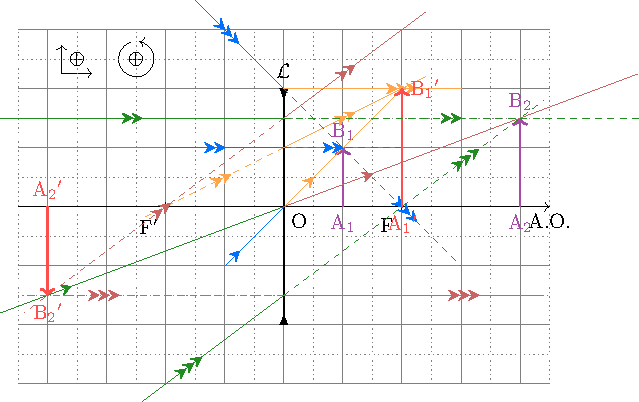
\includegraphics[width=.7\linewidth]{divCF}
			      \caption{Image réelle ou virtuelle pour une lentille divergente.}
			      \label{fig:divcf}
		      \end{figure}
	\end{enumerate}
}

\newpage
\exercice[52]{Instruments d'optique à l'infini \switch{\hfill -- Deux parties indépendantes -- \hfill}{\hfill \small D'après CCP PC 2015 \hfill}}
\restartlist{enumerate}

\subsection{Principe du téléobjectif}

\ifstudent{Dans un téléobjectif d'appareil photographique, une lentille
	convergente $\Lc_1$ est associée à une lentille divergente $\Lc_3$ dans le
	but de photographier un objet AB lumineux situé à l'infini. Le point
	objet A est choisi sur l'axe optique commun aux deux lentilles, et
	l'objet AB est orthogonal à l'axe. Le système est réglé pour que l'image
	finale $\ABp$ de $\AB$ se forme sur un capteur (P) orthogonal à l'axe et
	repéré par la position du point P, intersection de l'axe avec la plaque
	(voir figure~\ref{fig:teleobj_plain})~:

	\[
		\rm AB \opto{\Lc_1}{\rm O_1} \ABb \opto{\Lc_3}{\rm O_3} \ABp
	\]
}

\switch{
	\begin{enumerate}
		\item L'appareil est initialement déréglé et rendu afocal~: l'image $\ABp$
		      est renvoyé à l'infini. Déterminer, en fonction de $f'_1$ et $f'_3$ la
		      distance $\obar{\rm O_1O_3}$.

		\item Pour régler l'appareil afin que l'image définitive $\ABp$ se forme sur
		      la plaque (P), faut-il écarter ou rapprocher les deux lentilles l'une
		      de l'autre~?

		\item Compléter la figure~\ref{fig:teleobj_plain} en annexe, en traçant,
		      lorsque l'appareil est réglé, la marche d'un faisceau lumineux
		      incident, issu de B (situé à l'infini) et incliné d'un petit angle
		      $\alpha$ par rapport à l'axe optique. Préciser, sur ce schéma, la
		      position de l'image finale B$'$.
	\end{enumerate}
	On choisit $f'_1=+\SI{10,0}{cm}$ ;$f'_3=-\SI{3,0}{cm}$ ; $\obar{\rm
			O_3P}=+\SI{10,0}{cm}$ ; $\alpha=-\SI{0,10}{rad}$.
	\begin{enumerate}
		\item Déterminer la position de la lentille $\Lc_3$ en calculant la distance
		      $\obar{\rm F'_1F_3}$.
		\item Calculer la taille $\ABp$ de l'image portée sur la plaque (P).
	\end{enumerate}
}{
	\begin{enumerate}
		\item L'objet étant à l'infini, l'image intermédiaire  $\ABb$ est située
		      dans le plan focal image de la lentille $\Lc_1$. L'image finale $\ABp$
		      étant rejetée à l'infini, l'image intermédiaire $\ABb$ est aussi située
		      dans le plan focal objet de la lentille  $\Lc_3$. On en déduit que les
		      foyer image $F'_1$ et objet $F_3$ sont confondus~:

		      $A_{\infty} \xrightarrow{\left( L_1 \right)} A_1 =F'_1 =F_3
			      \xrightarrow{\left( L_3 \right)} A'_{\infty }$

		      On obtient donc $\obar{\rm O_1O_3} = \obar{\rm O_1F'_1} +\obar{\rm
				      F'_1F_3} + \obar{\rm F_3O_3} = \obar{\rm O_1F'_1} + \obar{\rm F_3O_3}$
		      d'où $\boxed{\obar{\rm O_1O_3} = f'_1 + f'_3}$

		\item La relation de conjugaison de \textsc{Descartes} appliquée à la lentille
		      $\Lc_3$ s'écrit $\frac{1}{\obar{\rm O_3A'}} - \frac{1}{\obar{\rm O_3A_1}}
			      = \frac{1}{f'_3}$. Pour amener l'image définitive sur la plaque, il faut
		      diminuer la distance $\obar{\rm O_3A'}$ et donc diminuer la distance
		      $\obar{\rm O_3A_1}=\obar{\rm O_3F'_1}$. Il faut donc rapprocher la
		      lentille $\Lc_3$ du plan focal image de la lentille $\Lc_1$ et donc
		      \xul{écarter les deux lentilles $\Lc_1$ et $\Lc_3$ l'une de l'autre}.
		\item On obtient la figure en annexe.
		\item D'après la formule de conjugaison de \textsc{Newton} appliquée à la lentille
		      $\Lc_3$~:

		      $\obar{\rm F_3A_1}.\obar{\rm F'_3A'} = - f'^2_3$ soit $\obar{\rm
				      F_3F'_1}.\obar{\rm F'_3P} = - f'^2_3$ d'où $\obar{\rm F'_1F_3} =
			      \frac{f'^2_3}{\obar{\rm F'_3P}} = \frac{f'^2_3}{\obar{\rm F'_3O_3} +
				      \obar{\rm O_3P}}$

		      On aboutit à $\boxed{\obar{\rm F'_1F_3} = \frac{f'^2_3}{\obar{\rm
						      O_3P} - f'_3}}$~: $\xul{\obar{\rm F'_1F_3} =
				      \SI{0.69}{\centi\meter}}$

		\item La taille de l'image intermédiaire est donnée par la relation
		      $\obar{\rm \ABb} = \alpha f'_1$ (en raisonnant dans le triangle
		      $O_1F'_1B_1$).

		      La taille de l'image définitive est donnée par la relation $\ABp =
			      \gamma_3 \obar{\rm \ABb} = \gamma_3 \alpha f'_1$.

		      $\gamma_3$ est le grandissement introduit par la lentille $\Lc_3$ dont
		      l'expression est donnée par la formule de \textsc{Newton}~: $\gamma_3 =
			      \frac{f'_3}{\obar{\rm F_3F'_1}} = - \frac{f'_3}{\obar{\rm F'_1F_3}}$.
		      On en déduit $\boxed{\ABp = - \frac{f'_3}{\obar{\rm F'_1F3}} \alpha
				      f'_1}$~: $\xul{\ABp = \SI{-4.3}{\centi\meter}}$.
	\end{enumerate}
}

\subsection{Principe de la lunette astronomique}
\ifstudent{
	La lunette astronomique est un système centré constitué d'un objectif et d'un
	oculaire. L'objectif est assimilé à une lentille mince convergente de centre
	optique O$_1$, de distance focale $f'_1$ et de diamètre $D_1$. L'oculaire est
	une lentille mince convergente de centre optique O$_2$, de distance focale
	$f'_2$ et de diamètre $D_2$.

	L'objectif donne, d'un objet éloigné, une image réelle appelée image
	objective. Cette dernière est observée au moyen de l'oculaire.
}

\switch{
	\begin{enumerate}
		\item À quelle condition l'œil d'un-e observateurice, supposé sans défaut,
          n'accommode pas~? En déduire la position relative de l'objectif et de
          l'oculaire. Ce système optique possède-t-il des foyers~? Comment se
          nomme un tel système optique~?
    \item Rappeler les conditions de \textsc{Gauss}. Réaliser un schéma, sans respecter
          les échelles, montrant le devenir d'un rayon incident faisant un angle
          $\tt$ avec l'axe optique et émergeant sous un angle $\tt'$ dans les
          conditions de \textsc{Gauss}.
		\item Déterminer l'expression du grossissement de la lunette
		      en fonction de $f'_1$ et $f'_2$ et calculer ce
		      grossissement si  $f'_1=\SI{1,0}{\meter}$ et $f'_2=\SI{20}{mm}$.
	\end{enumerate}
	On considère un faisceau lumineux issu d'un point objet $A$ à l'infini sur
	l'axe optique de la lunette (figure \ref{fig:lunette2}).
	\begin{enumerate}
		\item Compléter l'annexe et représenter le devenir d'un tel faisceau
		      lumineux limité par la monture de lentille objectif (encore appelée
		      diaphragme d'ouverture).
		\item Exprimer le diamètre $D$ du faisceau de rayons issu de l'oculaire en
		      fonction du grossissement $G$ de la lunette ainsi que du diamètre
		      $D_1$ du diaphragme d'ouverture.
		\item Après avoir calculé la valeur du diamètre $D$ du faisceau de rayons
		      issu de l'oculaire, montrer que c'est le diaphragme d'ouverture, de
		      diamètre $D_1$, qui limite et non l'oculaire de diamètre $D_2$. On
		      donne $D_1=\SI{10}{\centi\meter}$ et $D_2=\SI{6,0}{mm}$.
	\end{enumerate}
	On considère un objet ponctuel situé à l'infini en dehors de l'axe optique
	et dans la direction $\tt$ par rapport à ce dernier (figure
	\ref{fig:lunette3}).
	\begin{enumerate}
    \item Compléter l'annexe. On dit de la monture de l'oculaire qu'elle est le
          diaphragme de champ de la lunette. Pouvez-vous justifier cette
          affirmation~?
		\item L'objectif d'une lunette astronomique doit être capable de donner une
		      image parfaite d'un point infiniment éloigné. Pour cela, il doit,
		      notamment, être achromatique. D'où provient l'aberration chromatique
		      d'une lentille~? Comment, en physique, qualifie-t-on ce type de milieu
		      ~?
	\end{enumerate}
}{
	\begin{enumerate}
		\item \xul{L'observation à l'infini} se fait sans fatigue
		      d'accommodation. Il faut donc que l'image objective se forme dans le
		      plan focal objet de l'oculaire. La lunette visant un objet à l'infini
		      en forme une image objective dans le plan focal image de l'objectif~:
		      ainsi, \emph{le plan focal image de l'objectif est confondu avec le
			      plan focal objet de l'oculaire}.

		      Le système est \xul{afocal}, il n'a pas de foyers et il donne
		      d'un objet à l'infini une image finale rejetée à l'infini.

		\item Les rayons traversant un système optique centré dans les conditions de
		      \textsc{Gauss} sont \xul{paraxiaux}, c'est-à-dire peu écartés de l'axe
		      optique et peu inclinés par rapport à cet axe.
		      \begin{figure}[htbp]
			      \centering
			      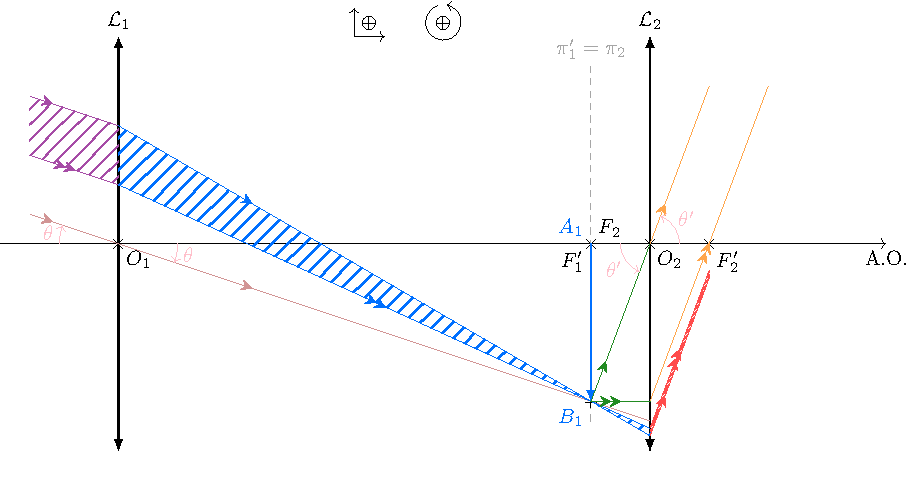
\includegraphics[width=.8\linewidth]{lunette1_corr}
			      % \label{fig:}
		      \end{figure}
		      On trace le rayon incident passant par le centre optique $O_1$ de
		      l'objectif, faisant un angle $\tt$ avec l'axe optique. Ce rayon
		      n'est pas dévié. Ce rayon arrive sur l'oculaire de façon quelconque.
		      On trace le rayon passant par $B_1$ et par $O_2$~: il ne sera pas
		      dévié. Or, comme $\ABb$ est dans le plan focal objet $\pi_2$, on sait
		      que tous les rayons passant par $B_1$ sortiront parallèle à celui-ci.
		      \smallbreak
		      Les deux rayons émergeant de l'oculaire sur le schéma ci-dessus sont
		      parallèles entre eux. Ils proviennent d'un même point objet qui est un
		      foyer secondaire objet pour l'oculaire, $B_1$.
		\item Le rayon incident forme un angle $\tt \ll \SI{1}{\radian}$ avec
		      l'axe optique. La lunette astronomique travaille dans les conditions
		      de \textsc{Gauss} donc $\tt' \ll \SI{1}{\radian}$ d'où $\tan{(\tt)} = \tt$ et
		      $\tan{(\tt')} = \tt'$.
		      \smallbreak
		      On a donc, en exprimant $\tan{(\tt)}$ et $\tan{(\tt')}$ dans les
		      triangles rectangles $\rm O_1F'_1B_1$ et $\rm O_2F_2B_1$~:
		      \smallbreak
		      \begin{gather*}
			      \tt = \frac{\ABb}{\obar{\rm O_1F_1'}}
			      \qet
			      \tt' = \frac{\ABb}{\obar{\rm O_2F_2}}
			      \qso
			      \boxed{G = -\frac{f_1'}{f_2}}
			      \qav
			      \left\{
			      \begin{array}{rcl}
				      f_1' & = & \SI{1e3}{mm}
				      \\
				      f_2' & = & \SI{20}{mm}
			      \end{array}
			      \right.\\
			      \AN
			      \xul{
				      G = -50
			      }
		      \end{gather*}
		\item Le faisceau incident parallèle à l'axe optique émerge de l'objectif en
		      convergeant vers le foyer principal image F$'_1$ de l'objectif. Comme
		      ce point est confondu avec l foyer principal objet F$_2$ de
		      l'oculaire, le faisceau émergent est un faisceau de rayons parallèles
		      à l'axe optique.

		\item On peut appliquer le théorème de Thalès dans les triangles $\rm
			      MO_1F'_1$ et $\rm F_2O_2Q$, ainsi~: $\frac{f'_2}{f'_1} = \frac{\rm
				      PQ}{2} / \frac{\rm MN}{2}$ soit encore $\frac{f'_2}{f'_1} =
			      \frac{D}{D_1}$.

		      On en conclut que $\boxed{D = \frac{D_1}{\abs{G}}}$
		\item On calcule~: $\xul{D = \SI{2.0}{mm}}$

		      Comme $D < D_2$, c'est bien le diamètre $D_1$ de l'objectif qui limite
		      le diamètre du faisceau émergent.

		\item On représente le chemin des rayons lumineux du faisceau incident
          incliné d'un angle $\tt$ plus important par rapport à l'axe optique
          (on suppose les conditions de \textsc{Gauss} toujours vérifiées)~: les
          rayons déviés par l'objectif convergent en un point du plan focal
          image de l'objectif (foyer secondaire image).
          \smallbreak
          On remarque que \xul{ces rayons ne frappent pas l'oculaire} car ils
          sont arrêtés par la monture. Ainsi, la monture de l'oculaire délimite
          la zone de l'espace objet qui peut donner une image par la lunette~:
          c'est \xul{le diaphragme de champ}.

		\item L'aberration chromatique d'une lentille provient du fait que
		      l'\xul{indice optique} du milieu la constituant dépend de la
			      \xul{longueur d'onde} de la radiation lumineuse considérée.

		      Le milieu constituant la lentille est un \xul{milieu dispersif}.
	\end{enumerate}
}

\newpage
\setcounter{section}{0}
\prblm[29]{Étude de pierres précieuses \ifprof{\hfill \small D'après CCP 2007 PC\hfill}}
\restartlist{enumerate}

\ifstudent{
	Une collectionneuse de gemmes possède trois petites pierres transparentes et
	incolores : une moissanite, un zircon et un morceau de verre à fort indice
	(flint), ainsi qu'un flacon de iodure de méthylène liquide. Les propriétés
	physiques de ces quatre substances, ainsi que celles du quartz, sont résumées
	dans le tableau ci-dessous.

	\begin{table}[htbp!]
		\centering
		\caption{Données}
		\begin{tabular}{lcc}
			\toprule
			Substance           & $\rho (\si{kg.m^{-3}})$ & $n$        \\
			\midrule
			Zircon              & \num{4690}              & \num{1,95} \\
			Moissanite          & \num{3210}              & \num{2,70} \\
			Verre flint         & \num{3740}              & \num{1,64} \\
			Quartz              & \num{2651}              & \num{1,55} \\
			Iodure de méthylène & \num{3330}              & \num{1,75} \\
			\bottomrule
		\end{tabular}
		\label{tab:gemdata}
	\end{table}

	Le zircon, la moissanite et le verre flint ont été mélangés, si bien que leur
	propriétaire doit à présent les identifier.
}

\subsection{Réfractomètre à réflexion interne totale}

\ifstudent{
	Pour mesurer l'indice de réfraction d'une pierre précieuse bien polie, on peut utiliser en gemmologie un réfractomètre à réflexion totale interne (RTI).
}

\switch{
	\begin{enumerate}
		\item \label{quest:il} On considère un milieu 1 d'indice $n_1$ et un milieu
          2 d'indice $n_2$ moins réfringent. Déterminer à quelle condition sur
            l'angle d'incidence, le rayon subit une réflexion totale à
            l'interface entre les deux milieux. Une explication efficace en
            français est attendue. Un schéma doit préciser la position des
            angles et des rayons par rapport à l'interface.
	\end{enumerate}

  Dans le cas du réfractomètre à RTI, les deux milieux utilisés sont un verre
  très dense optiquement ($n_v=1,96$) et la pierre précieuse (gemme) d'indice
  $n_g$ inconnu. La gemme est placée sur le verre comme représenté sur la figure
  \ref{fig:refractometre}. Sur une échelle graduée située à l'intérieur du
  réfractomètre apparaissent deux zones: une zone claire et une zone sombre.
  Lors de la lecture du réfractomètre, l'utilisateur repère la frontière entre
  les deux zones et lit la valeur d'indice sur les graduations.

	\begin{figure}[htbp]
		\centering
		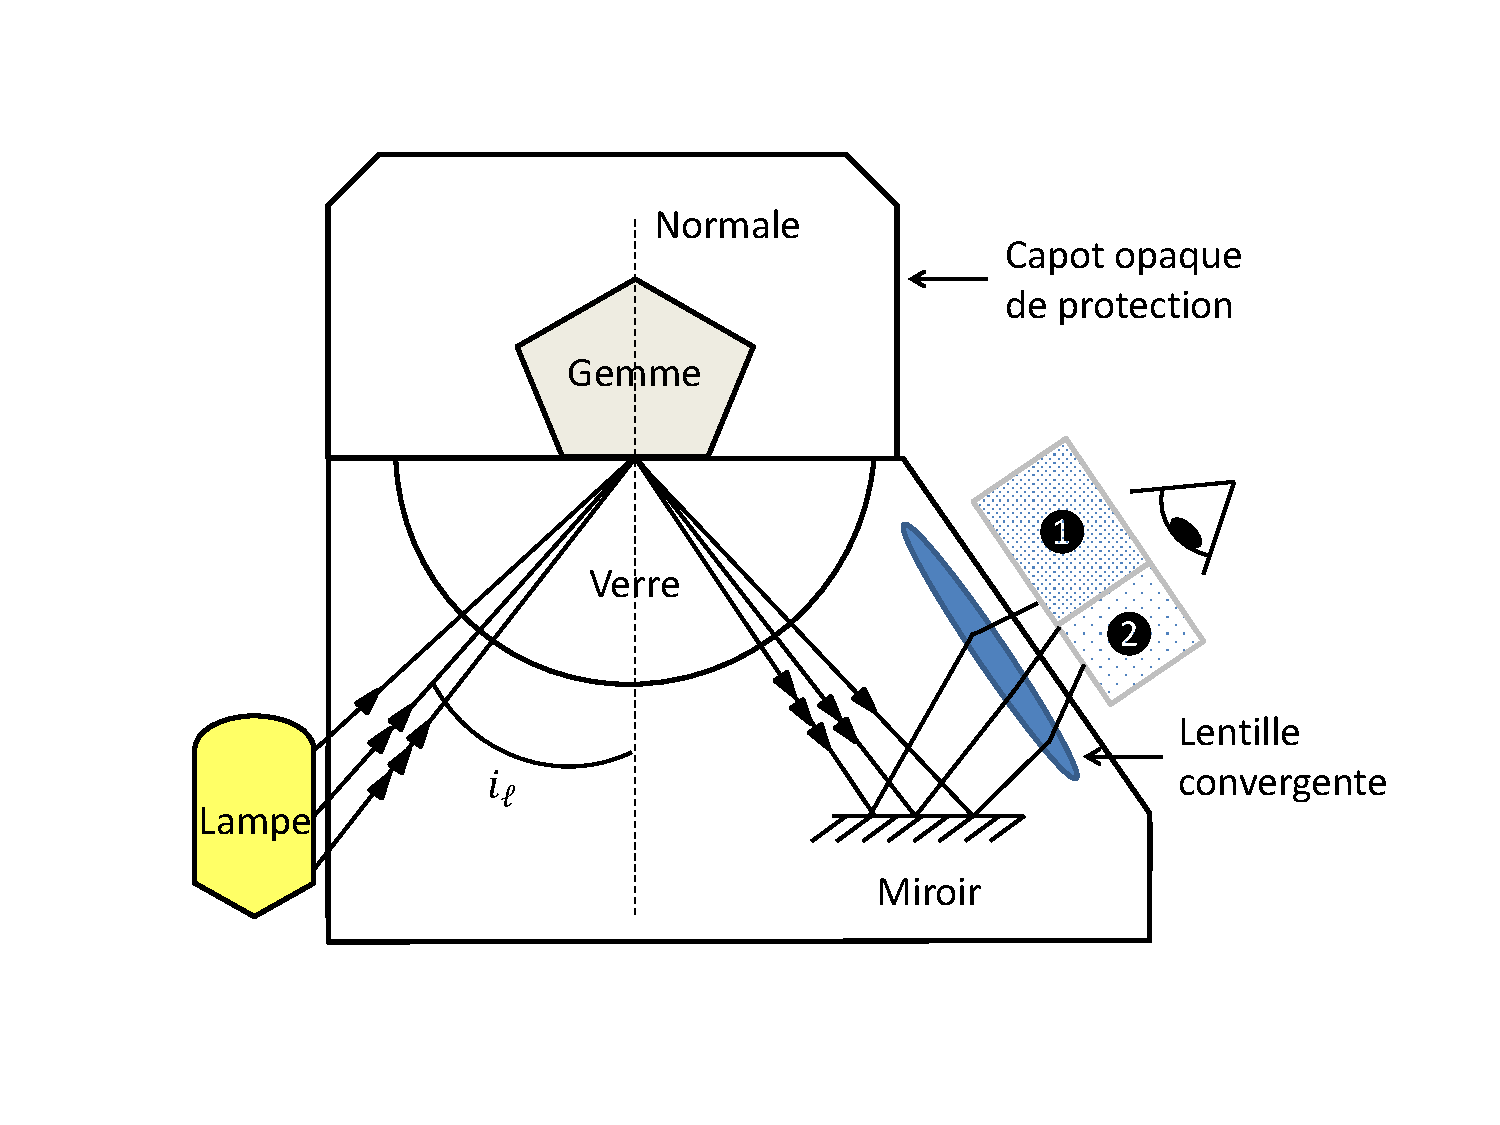
\includegraphics[width=.7\linewidth]{refractometre}
		\caption{Schéma du réfractomètre à RTI}
		\label{fig:refractometre}
	\end{figure}

	\begin{enumerate}
		\item Le réfractomètre ne peut pas être utilisé en lumière blanche car un
		      «~arc-en-ciel~» apparaît sur la zone graduée, rendant impossible toute
		      lecture. Quelle propriété du verre dense est mise ici en évidence~?
		\item Sur la figure \ref{fig:refractometre}, laquelle des zones 1 ou  2 est
		      la zone claire~? La zone sombre~? Justifier soigneusement.
		\item Quelle est la valeur de l'angle d'incidence qui marque la frontière
		      zone claire / zone sombre pour le quartz~?
		\item Le réfractomètre indique OTL (over the limit) pour une des 3 pierres
		      précieuses du collectionneur. Laquelle et pourquoi~?
	\end{enumerate}
}{
	\begin{enumerate}
		\item Comme $n_2<n_1$, le rayon réfracté est plus éloigné de la normale au
		      point d'incidence que le rayon incident. De ce fait, au delà d'un
		      angle d'incidence $i_{1\ell}$, le rayon réfracté n'existe plus~: il y
		      a réflexion totale. Pour déterminer $i_{1\ell}$, on se place dans la
		      situation où la réfraction est rasante et on utilise la loi de la
		      réfraction de \textsc{Snell-Descartes}~:
		      \[
			      n_1\sin(i_{1\ell})=n_2\sin(\pi/2)
			      \qso
			      \boxed{i_{1\ell}=\arcsin\left(\frac{n_2}{n_1}\right)}
		      \]
		      Ainsi, \xul{pour $i>i_{1\ell}$ le rayon est totalement
			      réfléchi.}%

		      \begin{figure}[htbp!]
			      \centering
			      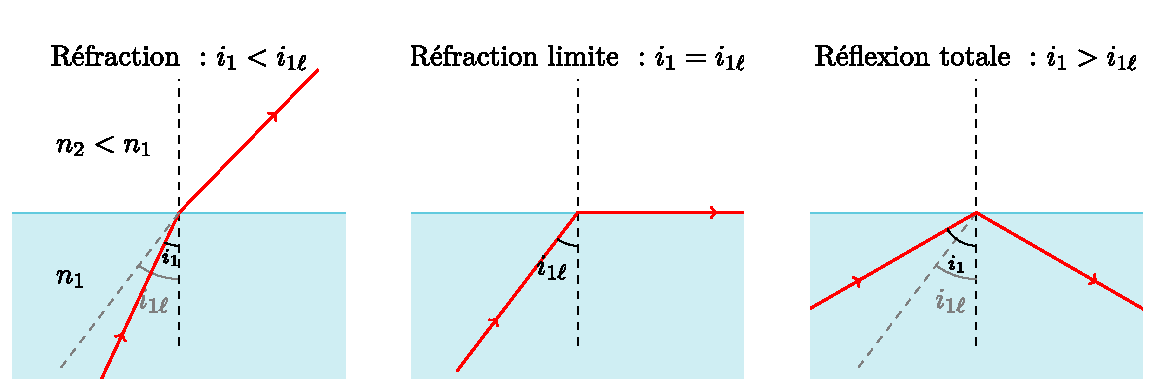
\includegraphics[width=.7\linewidth]{refraction_limite}
			      \label{fig:reflim}
		      \end{figure}
		\item Le spectre de la lumière blanche est «~étalé~» par le verre~: on met
		      en évidence le fait que le verre est un \xul{milieu dispersif.}
		\item La zone 1 est éclairée par les rayons d'angle d'incidence inférieur à
		      l'angle d'incidence limite de réflexion totale. Une partie de
		      l'énergie de ces rayons a donc été perdue par réfraction dans la gemme
		      avant d'arriver jusqu'à la zone graduée. La zone 2 est éclairée par
		      des rayons qui ont subi une réflexion totale sur la gemme: aucune
		      énergie lumineuse n'a été perdue dans la gemme.
		      \smallbreak
		      \xul{La zone 1 est donc la zone sombre et la zone 2 est la zone
			      claire.}
		\item L'angle d'incidence qui marque la limite entre les deux zones est
		      l'angle limite de réfraction. On utilise donc le résultat de la
		      question~1 avec $n_1=n_v=\num{1.96}$ et $n_2=n_g=\num{1.55}$~:
		      \[
			      \xul{i_\ell=\ang{52.3}}
		      \]
		\item Pour la moissanite, $n_g>n_v$ il n'y a donc plus de réflexion totale
		      possible sur la face inférieure de la gemme: il y a toujours
		      réfraction et réflexion en même temps. Ainsi, il n'existe plus de zone
		      nettement plus sombre : \xul{le réfractomètre ne peut pas être
			      utilisé pour la moissanite.}
	\end{enumerate}
}

\subsection{Identification qualitative de pierres précieuses}

\ifstudent{En l'absence de réfractomètre, la collectionneuse peut tout de même
	identifier les trois gemmes.}

\switch{
	\begin{enumerate}
		\item L'immersion des trois pierres dans le iodure de méthylène, permet de
		      reconnaître immédiatement l'une des trois pierres. Laquelle~?
	\end{enumerate}
}{
	\begin{enumerate}
		\item La moissanite a une masse volumique plus faible que celle du liquide
		      contrairement aux deux autres~: elle va donc être la seule à flotter.
		      \xul{Ceci permet d'identifier immédiatement la moissanite.}
	\end{enumerate}
}

\ifstudent{Les deux pierres restantes sont posées sur un morceau de verre
	dépoli, recouvertes de iodure de méthylène d'indice $n_{\rm liq}$, puis
	éclairées depuis le haut. un miroir incliné situé sous le verre  dépoli
	permet d'observer le verre dépoli par en dessous, comme représenté sur la
	figure \ref{fig:depoli}. La pierre numéro 1 est entourée d'un contour
	brillant, et ses arêtes vives sont sombres. La pierre numéro 2 est entourée
	d'un contour sombre et ses arêtes paraissent brillantes (figure
	\ref{fig:aretes}).

	\begin{figure}[htbp!]
		\centering
		\subcaptionbox{Dispositif expérimental\label{fig:depoli}}[.48\linewidth]
		{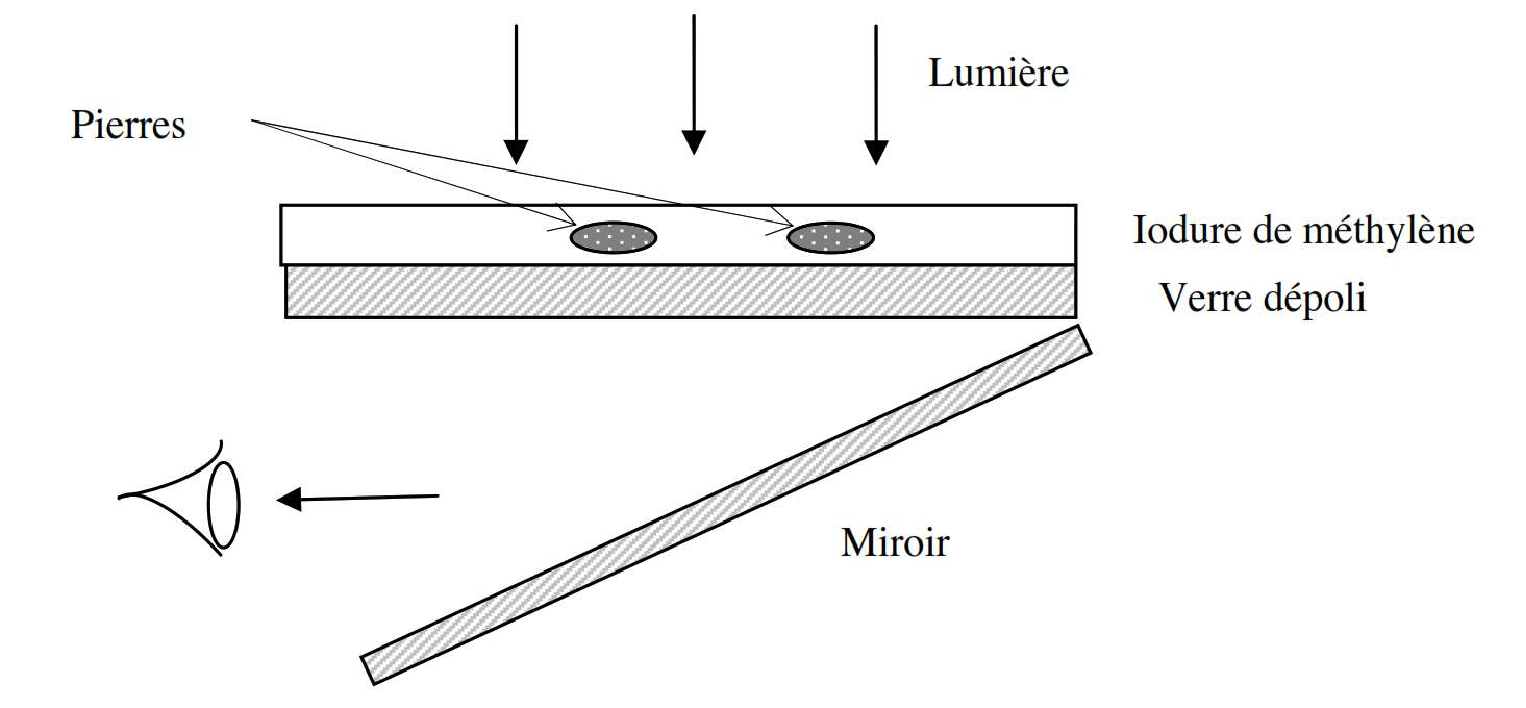
\includegraphics[width=\linewidth]{observation_depoli}}
		\subcaptionbox{Observations des gemmes\label{fig:aretes}}[.48\linewidth]
		{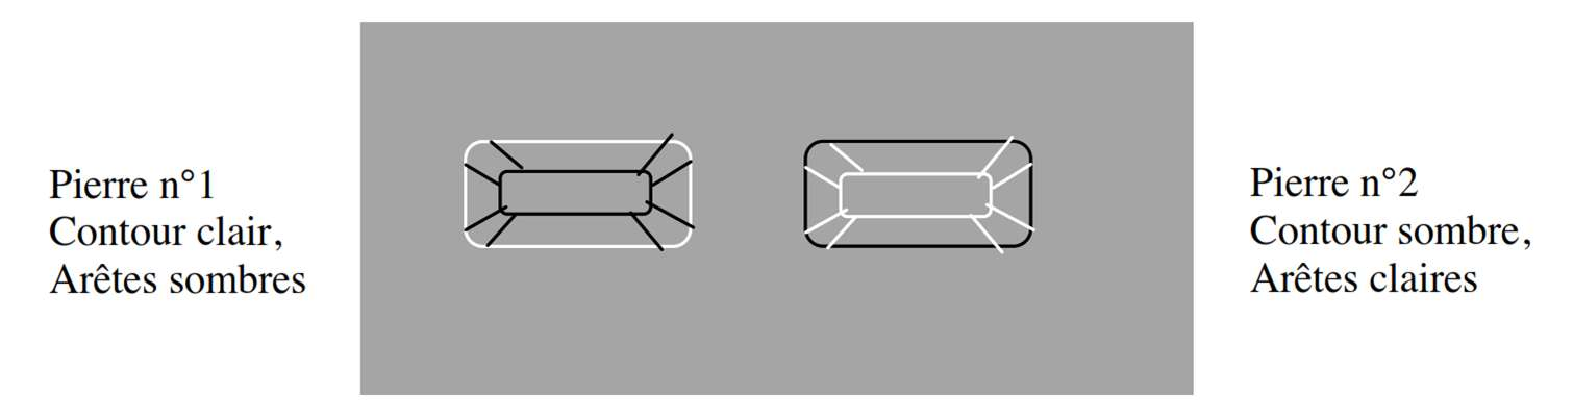
\includegraphics[width=\linewidth]{observation_gemmes}}
		\caption{}
		\label{fig:dispo}
	\end{figure}
}

\switch{
	\begin{enumerate}
		\item \textbf{(Annexe)} Sur la figure \ref{fig:gemme_e1} de l'annexe, tracer
          l'allure du prolongement des rayons réfractés issus de $\mathrm{A},
          \mathrm{B}, \mathrm{C}$ et $\mathrm{D}$, jusqu'à l'écran, dans le cas
          où l'indice de réfraction de la gemme $n_g$ est supérieur à $n_{\rm
          liq}$. Faire de même sur la figure \ref{fig:gemme_e2} dans le cas où
          l'indice de réfraction $n_g$ est inférieur à $n_{\rm liq}$. On ne
          tiendra pas compte des rayons réfléchis.
		\item En déduire, dans les deux cas, les zones de plus forte et de plus
		      faible intensité lumineuse sur l'écran. Identifier les pierres numéro
		      1 et numéro 2.
	\end{enumerate}

}{
	\begin{enumerate}
		\item On obtient les figures proposées en annexe en se rappelant qu'en
		      entrant dans un milieu plus réfringent que le milieu incident, les
		      rayons se rapprochent de la normale (et inversement si le milieu est
		      moins réfringent).
		\item On constate que, dans le cas $n_g>n_{\rm liq}$, la lumière se
		      concentre sous les arêtes (zones de forte intensité) et s'éloigne des
		      bords (zones de faible intensité). Dans le cas $n_g<n_{\rm liq}$,
		      la lumière s'éloigne des arêtes (zones de faible intensité) mais reste
		      sous les bords (zones de forte intensité).
		      \smallbreak
		      \xul{On en déduit que la pierre numéro 1 correspond au cas où
		      $n_g<n_{\rm liq}$~: c'est donc le verre flint (1,64<1,75).}
		      \smallbreak
		      \xul{Inversement la pierre numéro 2 correspond au cas où $n_g<n_{\rm
			      liq}$~: c'est donc le zircon (1,95>1,75).}
	\end{enumerate}
}

\newpage
\prblm[32]{Image au fond d'un gobelet \ifprof{\hfill \small D'après CCP 2012 PC \hfill}}
\restartlist{enumerate}

\ifstudent{
	Il existe de petits gobelets amusants (figure~\ref{fig:gobelet}~(a)) possédant
	la propriété suivante~:
	\begin{itemize}
		\item en l'absence de liquide, le fond du gobelet est constitué d'une
		      lentille sphérique qui ne laisse rien apparaître
		      (figure~\ref{fig:gobelet}~(b)) ;
		\item en présence de liquide, une image nette apparaît
		      (figure~\ref{fig:gobelet}~(c)).
	\end{itemize}

	\begin{figure}[htbp!]
		\centering
		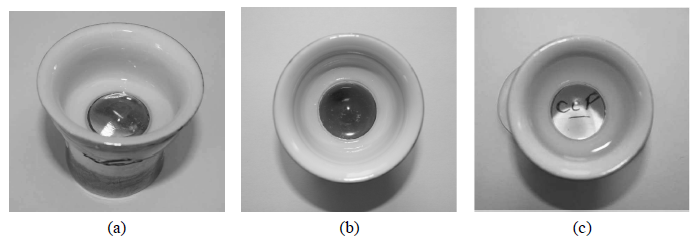
\includegraphics[width=.8\linewidth]{gobelets}
		\caption{}
		\label{fig:gobelet}
	\end{figure}

  L'objet de ce problème est de proposer une modélisation simple de ce phénomène
  optique. Les conditions de l'optique de \textsc{Gauss} seront supposées
  satisfaites tout au long du problème. Les figures ne sont pas à l'échelle. Les
  valeurs numériques considérées dans ce problème sont réalistes.
L'approximation des lentilles minces n'est, en revanche, pas vraiment justifiée
dans le contexte. }

\subsection{Visibilité d'un objet situé dans le plan focal objet}
\ifstudent{

  Sur un banc d'optique (figure~\ref{fig:montage1}) sont alignés un objet plan
  BB$'$, coupant l'axe optique en un point A et une lentille mince convergente
  $\Lc_1$ située au point S. B et B$'$ sont symétriques l'un de l'autre par
  rapport à l'axe optique. La figure représente le foyer principal objet F,
  confondu avec A, ainsi que le foyer principal image F'. L'œil d'une
  observatrice est placé en un point O de l'axe optique.
  \smallbreak
  La pupille de l'œil est représentée comme un disque centré en O, de diamètre
  PP$'$. Le bord de la lentille est un cercle, assimilable à un diaphragme
  DD$'$. Le diamètre de l'objet BB$'$ est identique à celui du diaphragme D$D'$.

	Données~: $\obar{\rm SA}=\SI{-12}{mm},
		\obar{\rm SO}=\SI{200}{mm},
		\obar{\rm BB'}=\obar{\rm DD'}=\SI{20}{mm},
		\obar{\rm PP'}=\SI{6}{mm}$

	\figsvgCap{P1/fig2.pdf_tex}{Montage de la lentille $\Lc_1$ (échelle non respectée).\label{fig:montage1}}
}

\switch{
	\begin{enumerate}
    \item Rappeler les hypothèses de l'approximation de \textsc{Gauss} en
          optique géométrique.

    \item Sur le document réponse \ref{fig:gob1}, construire graphiquement
		      l'allure de deux rayons issus de B et traversant la lentille. Faire
		      de même avec deux rayons issus de B$'$.

    \item Lorsque l'objet est situé dans le plan focal objet de la lentille,
          l'image se forme à l'infini et seule une fraction minime des rayons
          issus de l'objet est captée par la pupille de l'œil PP$'$. Il s'agit
          d'estimer cette fraction.
          \smallbreak
          Sur le document réponse \ref{fig:gob2}, tracer les rayons incidents
          correspondant aux rayons émergents DP$'$ et D$'$P. Placer les points
          objets E et E$'$, avec E en-dessous de l'axe optique.

		\item À l'aide du schéma précédent, déduire l'expression de la distance
      $\obar{\rm EE'}$ en fonction des distances $\obar{\rm SF}$, $\obar{\rm
      SO}$, $\obar{\rm DD'}$ et $\obar{\rm PP'}$. Calculer numériquement
      $\obar{\rm EE'}$.
      Puis donner la fraction d'aire, définie par le rapport $\tau_1 =
      (\rm EE'/BB')^2$, de l'objet visible par l'œil placé au point O.
	\end{enumerate}
}{
	\begin{enumerate}
    \item Dans l'approximation de \textsc{Gauss}, on ne considère que les rayons
          paraxiaux, c'est-à-dire les rayons proches de l'axe optique et
          faiblement inclinés par rapport à l'axe optique.
		\item Voir Annexe.
		\item Voir Annexe.
		\item Dans le triangle $SAE'$ rectangle en $A$~:
		      $\tan(\alpha)=\frac{EE'}{2SF}$

		      Dans le triangle $KDP'$ rectangle en $K$~:
		      $\tan(\alpha)=\frac{DD'+PP'}{2SO}$

		      On en déduit
		      \[
			      \boxed{EE'=\frac{(DD'+PP')\cdot SF}{SO}=\SI{1,56}{mm}
				      \quad;\quad \tau_1=6\cdot 10^{-3}}
		      \]
	\end{enumerate}
}

\subsection{Visibilité d'un objet situé entre le plan focal et la lentille}
\ifstudent{
	\figsvgCap{P1/fig3.pdf_tex}{Montage de la lentille $\Lc_2$ (échelle non respectée). \label{fig:montage2}}

  La figure~\ref{fig:montage2} représente un montage analogue à celui de la
  figure~\ref{fig:montage1}. La lentille $\Lc_1$ a été remplacée par une
  lentille $\Lc_2$ moins convergente. L'objet BB$'$ coupe l'axe en un point A
  distinct du foyer principal objet F. La distance $\obar{\rm SA}$ est encore
  égale à \SI{-12}{mm}, tandis que la distance focale $f' =\obar{\rm SF'}$ de la
lentille $L_2$ est désormais de \SI{36}{mm} (figure~\ref{fig:montage2}). }

\switch{
	\begin{enumerate}
    \item Déterminer par le calcul la position de l'image $\rm B_2B_2'$ de
          l'objet $\rm BB'$. Calculer le grandissement $\gamma=\obar{\rm
          B_2B'_2}/\obar{\rm BB'}$ et la taille de l'image $\rm B_2B'_2$.
          L'image est-elle réelle ou virtuelle~?
		\item Vérifier vos résultats en effectuant le tracé de rayons sur le
          document réponse \ref{fig:gob3}. Un carreau horizontal correspond à
          \SI{9}{mm}, et un carreau vertical à \SI{10}{mm}.

		\item Calculer la distance entre l'œil et le plan image $\rm B_2B'_2$. En
          déduire que le diaphragme $\rm DD'$ masque une partie de l'image $\rm
          B_2B'_2$ à l'observateur dont l'œil est situé en $\rm O$.

		      Estimer, dans l'approximation où les points O, P et P$'$ sont
		      confondus, la fraction surfacique $\tau_2$ de l'image $\rm B_2B'_2$
		      visible par l'œil de l'observateur situé en O.
	\end{enumerate}
}{
	\begin{enumerate}
		\item On note A$_2$, l'image de A à travers la lentille. D'après la
          relation de conjugaison de \textsc{Descartes}
		      \[
			      \frac{1}{\obar{\rm SA_2}}-\frac{1}{\obar{\rm SA}}=\frac{1}{f'}
			      \quad \Lra \quad
			      \boxed{\obar{\rm SA_2}=
				      \frac{f'\cdot\obar{\rm SA}}{f'+\obar{\rm SA}}=\SI{-18}{mm}}
		      \]

		      $\obar{\rm SA_2}<0$, donc l'image est virtuelle, ce qui est normal car
		      l'objet est dans la «~zone loupe~» de la lentille convergente,
		      c'est-à-dire entre le foyer objet principal objet et la lentille.

		      D'après la relation du grandissement de \textsc{Descartes},
		      \[
			      \boxed{\gamma=\frac{\obar{\rm SA_2}}{\obar{\rm SA}}=\num{1.5}}
		      \]

          On en déduit $\boxed{\obar{\rm B_2B'_2}=\gamma \obar{\rm
          BB'}=\SI{30}{mm}}$.

    \item On a bien $\obar{\rm SA_2}=\SI{-18}{mm}$. L'image est virtuelle et est
          \num{1.5} fois plus grande.

		\item La distance entre l'œil et le plan image $B_2B'_2$ est
		      $\boxed{\obar{\rm A_2O}=\SI{218}{mm}}$.

		      Soient $C$ et $C'$ les points extrêmes de l'image $B_2B'_2$ visible
		      depuis $O$. Les triangles $ODD'$ et $OCC'$ sont semblables, donc
		      d'après Thalès~:
		      \[
			      \boxed{CC'=\frac{A_2O}{SO}\times DD'=\SI{21,8}{mm}}
		      \]
		      On constate que $CC'<B_2B'_2$, donc on ne voit qu'une partie de
		      l'image.
		      \smallbreak
		      On en déduit $\boxed{\tau_2=\left (\frac{CC'}{B_2B'_2}  \right
				      )^2=0,53}$.
	\end{enumerate}
}

\subsection{Distance focale de lentilles minces accolées}

\ifstudent{

	Le modèle proposé pour décrire la situation représentée sur la
	figure~\ref{fig:gobelet}~(b) (absence de liquide) est celui d'une lentille
	mince plan-convexe de rayon de courbure $R$
	(figure~\ref{fig:association}~(a)). La lentille est constituée de verre
	d'indice $n_2$ entourée d'air d'indice $n_1$. Le modèle proposé pour décrire
	la situation représentée sur la figure~\ref{fig:gobelet}~(c) (présence de
	liquide) est la succession d'un dioptre plan entre un milieu d'indice $n_1$ et
	d'indice $n_2$, d'un dioptre sphérique de rayon de courbure $R$ entre un
	milieu d'indice $n_2$ et un milieu d'indice $n_3$, puis d'un second dioptre
	plan entre le milieu d'indice $n_3$ et le milieu d'indice $n_1$
	(figure~\ref{fig:association}~(b)).

	\begin{figure}[htbp!]
		\centering
		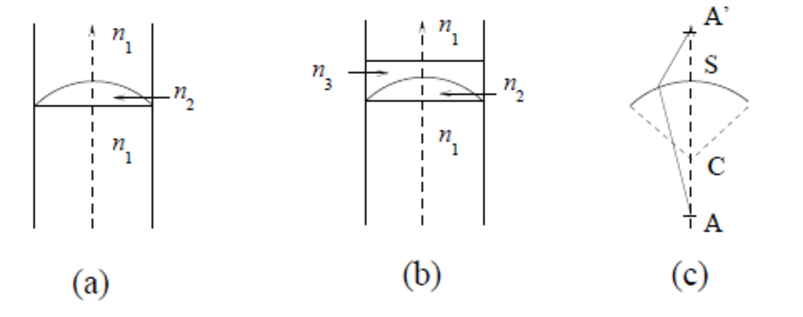
\includegraphics[width=.7\linewidth]{fig4}
		\caption{(a)~: Gobelet sans liquide ; (b) Gobelet avec liquide}
		\label{fig:association}
	\end{figure}
}

\switch{
	\begin{enumerate}
		\item On donne la formule de conjugaison correspondant à la succession de
		      dioptres représentés sur la figure~\ref{fig:association}~(a)
		      \[
			      n_1\left(\frac{1}{\obar{\rm SA'}}-\frac{1}{\obar{\rm SA}} \right) =
			      \frac{n_2-n_1}{\obar{\rm CS}}
		      \]
		      où $\obar{\rm CS}$ représente la distance algébrique entre le centre
		      de courbure et le sommet du dioptre sphérique, représenté sur
		      lafigure~\ref{fig:association}~(c).

		      Reconnaître la distance focale $f'_1$ de la lentille convexe dans
		      l'expression ci-dessus et calculer sa valeur numérique.

		      Données~: $n_1 = 1,00$, $n_2 = 1, 50$ et $R = \SI{6,0}{mm}$.

		\item On donne la formule de conjugaison correspondant à la succession de
		      dioptres représentés sur la figure~\ref{fig:association}~(b)~:
		      \[
			      n_1\left(\frac{1}{\obar{\rm SA'}}-\frac{1}{\obar{\rm SA}}\right) =
			      \frac{n_2-n_3}{\obar{\rm CS}}
		      \]
		      où $\obar{\rm CS}$ représente la distance algébrique entre le centre
		      de courbure et le sommet du dioptre sphérique, représenté sur la
		      figure~\ref{fig:association}~(c).

		      Reconnaître la distance focale $f'_2$ de la lentille plane dans
		      l'expression ci-dessus et calculer sa valeur numérique.

		      Données~: $n_1 = 1,00$, $n_2 = 1,50$, $n_3 = 1,33$ et $R =
			      \SI{6,0}{mm}$.

		\item L'objet à observer est situé à une distance de \SI{12}{mm} sous la
		      lentille (voir figure~\ref{fig:coupe}). Pourquoi ne voit-on rien en
		      l'absence de liquide~? Pourquoi l'image devient-elle visible lorsque
		      l'on remplit le verre~?
		      \begin{figure}[htbp]
			      \centering
			      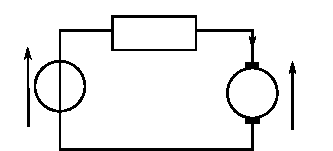
\includegraphics[width=.45\linewidth]{fig5}
			      \caption{Vue de coupe du gobelet.}
			      \label{fig:coupe}
		      \end{figure}
	\end{enumerate}
}{
	\begin{enumerate}
    \item Par identification avec la relation de conjugaison de
          \textsc{Descartes} en posant $S$ le centre optique de la lentille,
		      \[
			      \boxed{f'_1=\frac{n_1\obar{\rm CS}}{n_2-n_1}=\SI{12}{mm}}
		      \]
		\item De même, $\boxed{f'_2=\frac{n_1\obar{\rm CS}}{n_2-n_3}=\SI{35}{mm}}$.
		\item Dans ce qui précède, sans liquide, il n'y a que 0,6\% de la surface de
		      l'image $B_2B'_2$ visible, tandis qu'avec le liquide il y en a 53\%. Donc
		      l'image devient visible.
	\end{enumerate}
}

\switch{
	\newpage
	\chapter*{Annexe~: exercice 2}
	\begin{tikzpicture}[remember picture, overlay]
    \node[anchor=north west, align=left] at ([shift={(1.5cm,0)}]current page.north west)
		{\\[5pt]\Large\bfseries Nom~:\\[10pt]\Large\bfseries Prénom~:};
    \node[anchor=north east, align=right] at ([shift={(-1.5cm,-17pt)}]current page.north east)
    {\Large\bfseries Copie\hspace{.5cm}/\hspace{.5cm}};
	\end{tikzpicture}

	\begin{figure}[htbp!]
		\centering
		\subcaptionbox{Téléobjectif\label{fig:teleobj_plain}}
		[.80\linewidth]
		{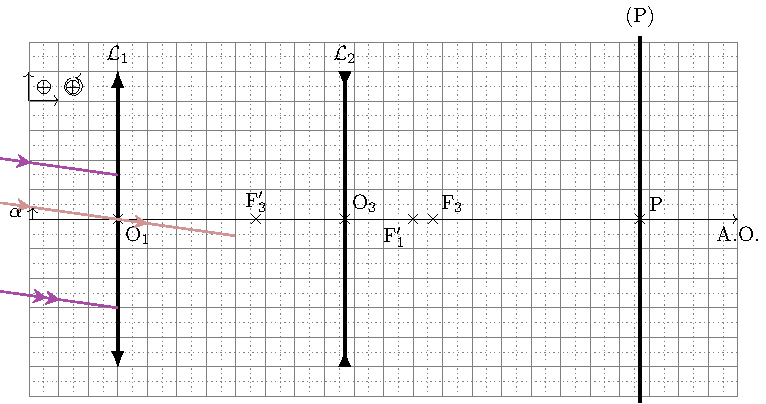
\includegraphics[width=\linewidth]{teleobj_plain}}
		\subcaptionbox{Rayons de l'infini parallèles\label{fig:lunette2}}
		[.80\linewidth]
		{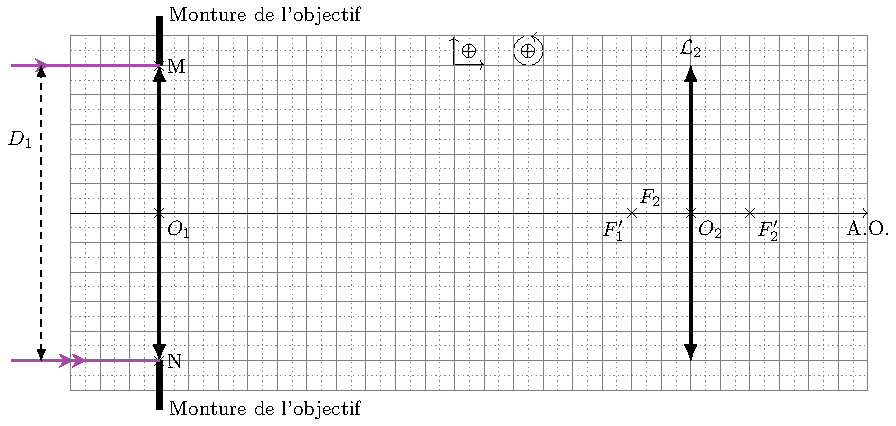
\includegraphics[width=\linewidth]{lunette2_enon}}
		\subcaptionbox{Rayons de l'infini avec un angle\label{fig:lunette3}}
		[.80\linewidth]
		{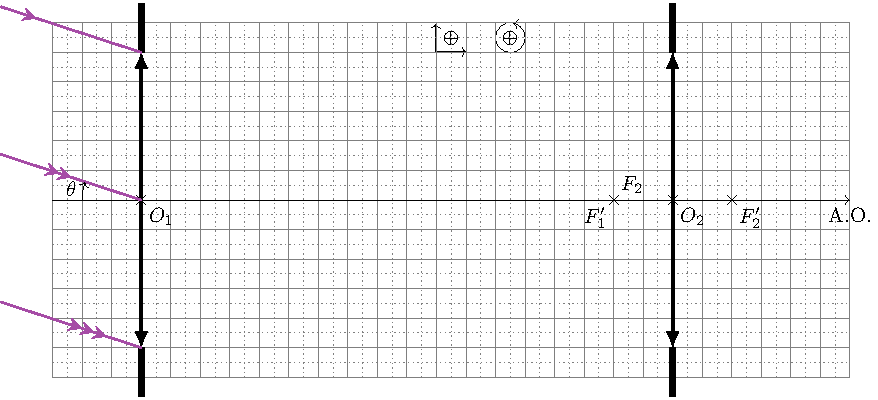
\includegraphics[width=\linewidth]{lunette3_enon}}
		\caption{}
		\label{fig:lunettes}
	\end{figure}

	\newpage
	\chapter*{Annexe~: problème 1}
	\begin{figure}[htbp]
		\centering
		\subcaptionbox{Cas où $n_g>n_{\rm liq}$\label{fig:gemme_e1}}
		{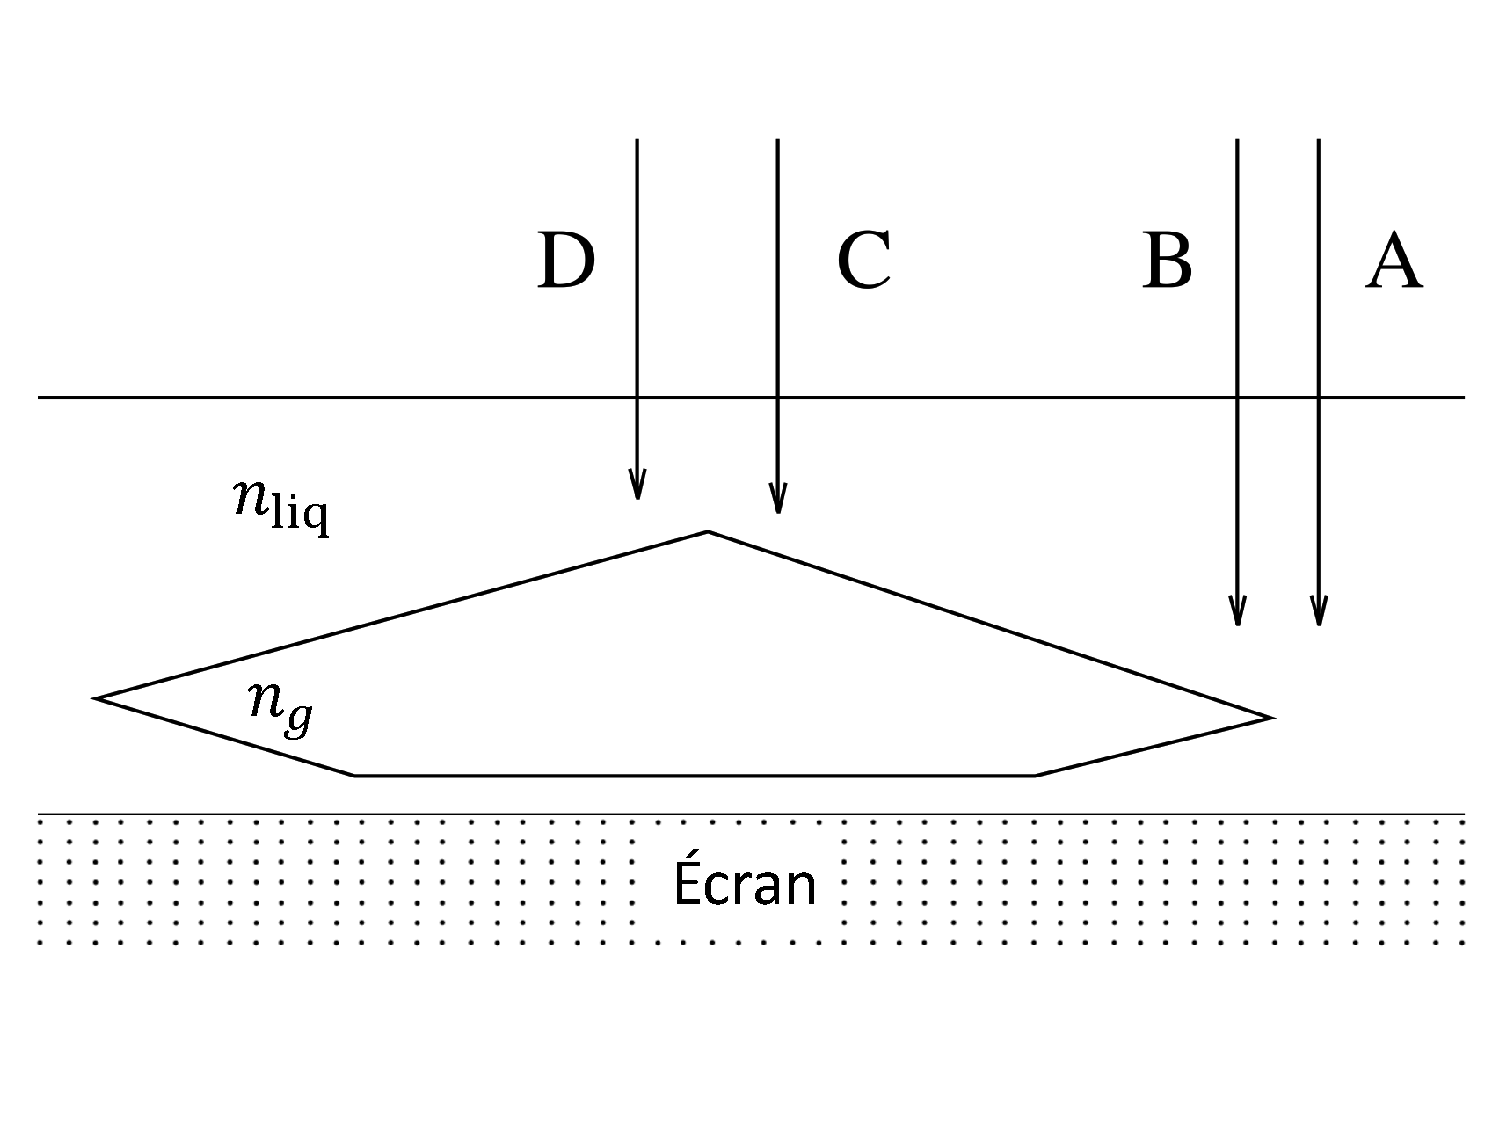
\includegraphics[width=.7\linewidth]{gemme_e}}
		\subcaptionbox{Cas où $n_g<n_{\rm liq}$\label{fig:gemme_e2}}
		{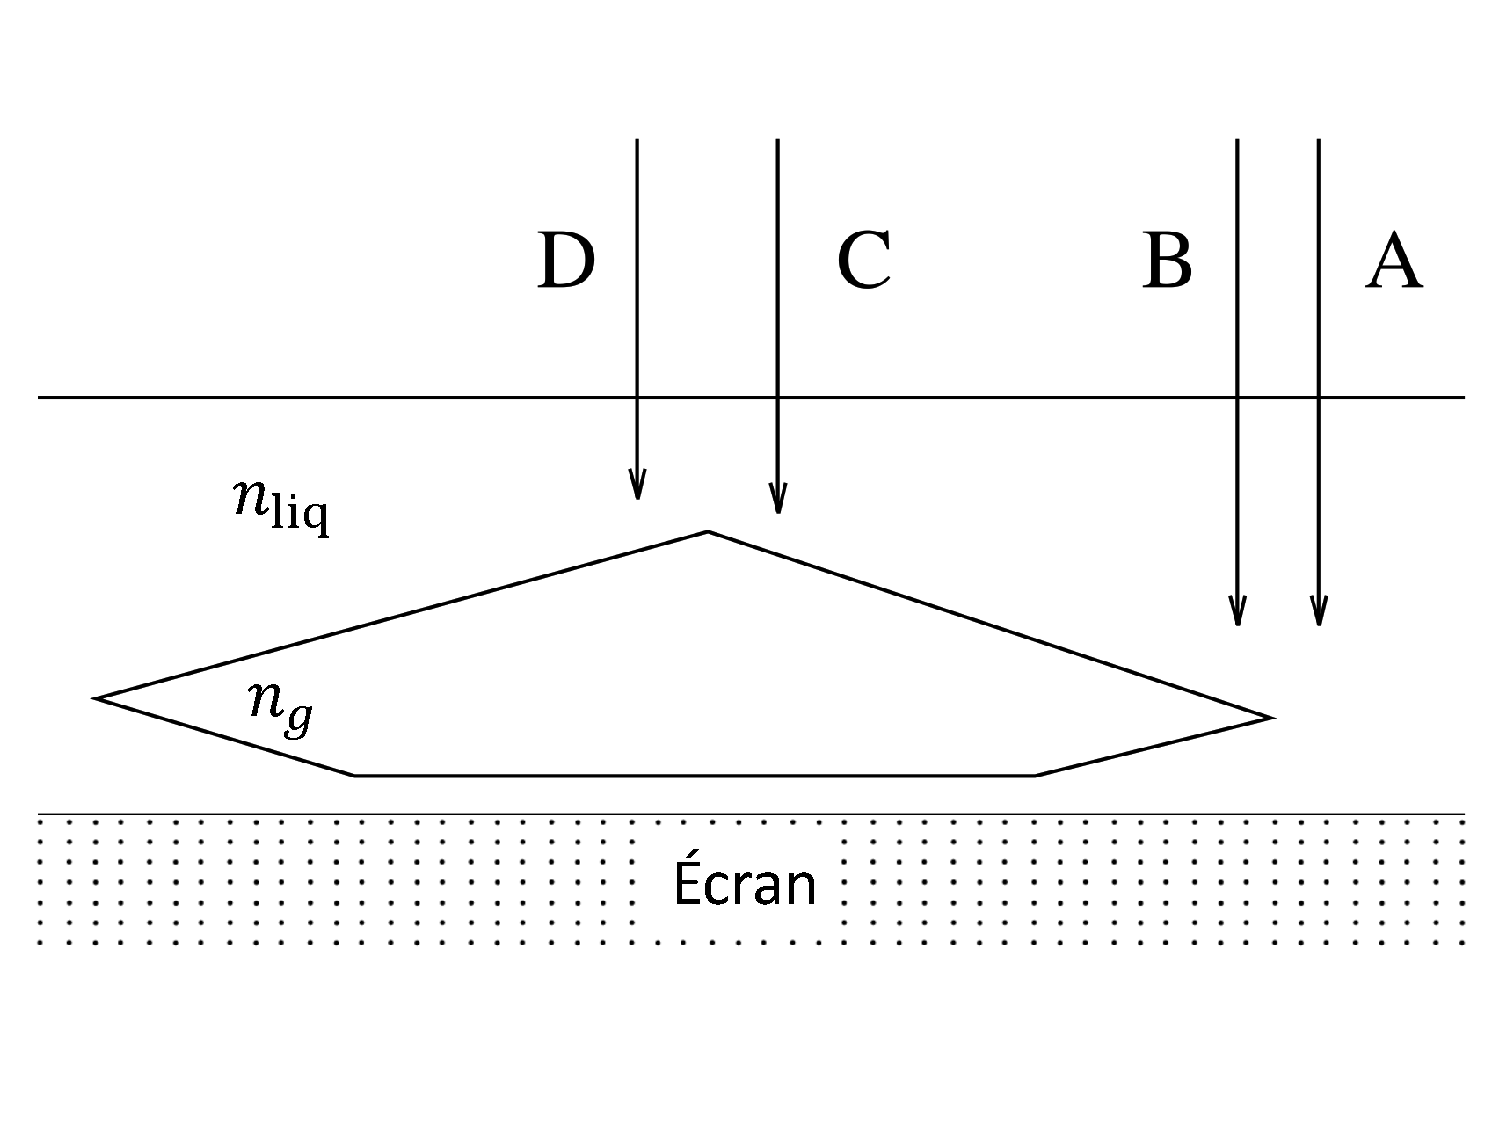
\includegraphics[width=.7\linewidth]{gemme_e}}
		\caption{}
	\end{figure}

	\newpage
	\chapter*{Annexe~: problème 2}
	\begin{tikzpicture}[remember picture, overlay]
    \node[anchor=north west, align=left] at ([shift={(1.5cm,0)}]current page.north west)
		{\\[5pt]\Large\bfseries Nom~:\\[10pt]\Large\bfseries Prénom~:};
    \node[anchor=north east, align=right] at ([shift={(-1.5cm,-17pt)}]current page.north east)
    {\Large\bfseries Copie\hspace{.5cm}/\hspace{.5cm}};
	\end{tikzpicture}
	\begin{figure}[htbp!]
		\centering
		\subcaptionbox{Annexe question 2\label{fig:gob1}}
		[.75\linewidth]
		{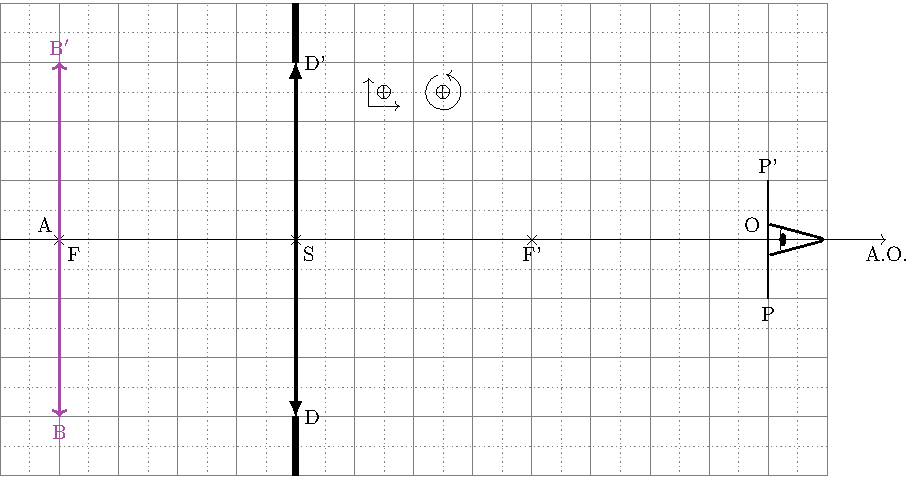
\includegraphics[width=\linewidth]{P1_1-enon}}
		\subcaptionbox{Annexe question 6\label{fig:gob2}}
		[.75\linewidth]
		{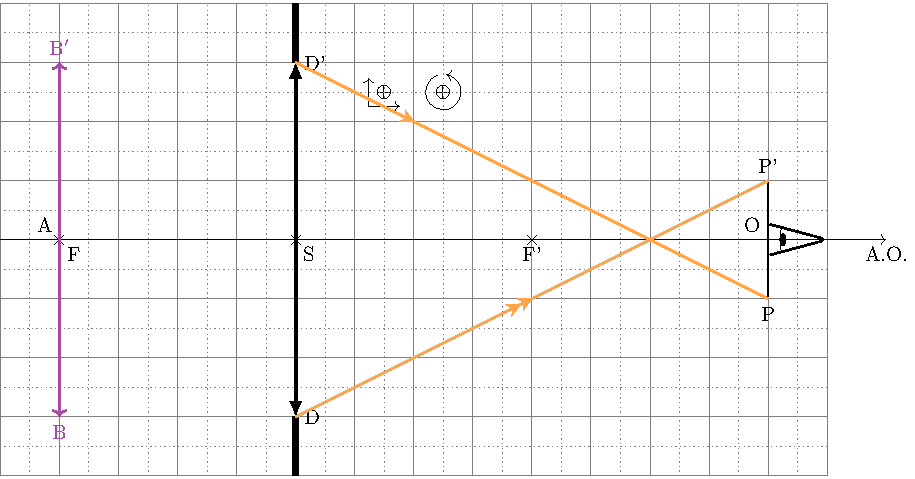
\includegraphics[width=\linewidth]{P1_2-enon}}
		\subcaptionbox{Annexe question 9\label{fig:gob3}}
		[.75\linewidth]
		{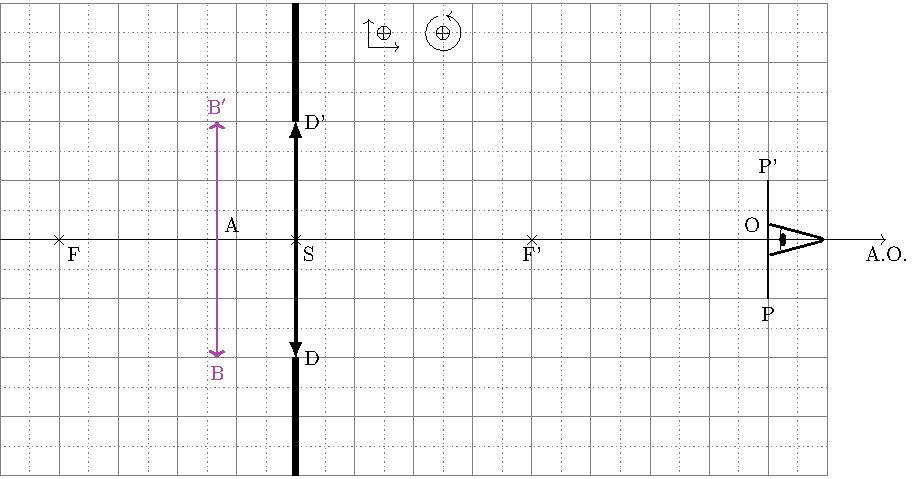
\includegraphics[width=\linewidth]{P1_3-enon}}
		\caption{}
		\label{fig:gob}
	\end{figure}

}{
	\newpage
	\chapter*{Annexe~: exercice 2}
	\begin{figure}[htbp!]
		\centering
		\subcaptionbox{Téléobjectif\label{fig:teleobj_plain}}
		[.80\linewidth]
		{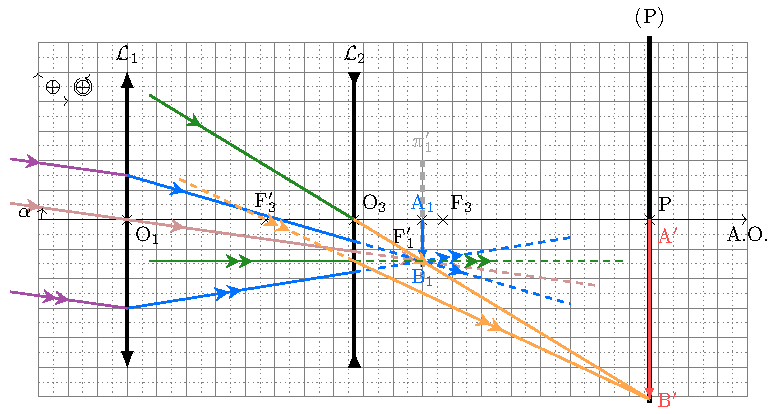
\includegraphics[width=\linewidth]{teleobj}}
		\subcaptionbox{Rayons de l'infini parallèles\label{fig:lunette2}}
		[.80\linewidth]
		{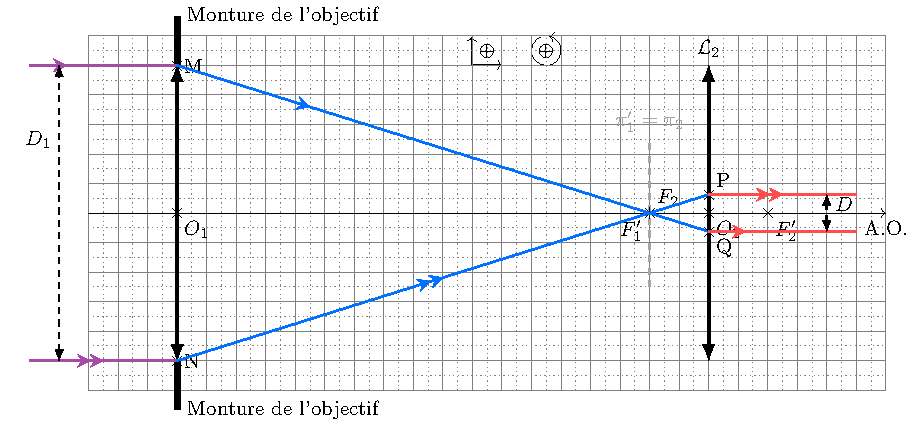
\includegraphics[width=\linewidth]{lunette2_corr}}
		\subcaptionbox{Rayons de l'infini avec un angle\label{fig:lunette3}}
		[.80\linewidth]
		{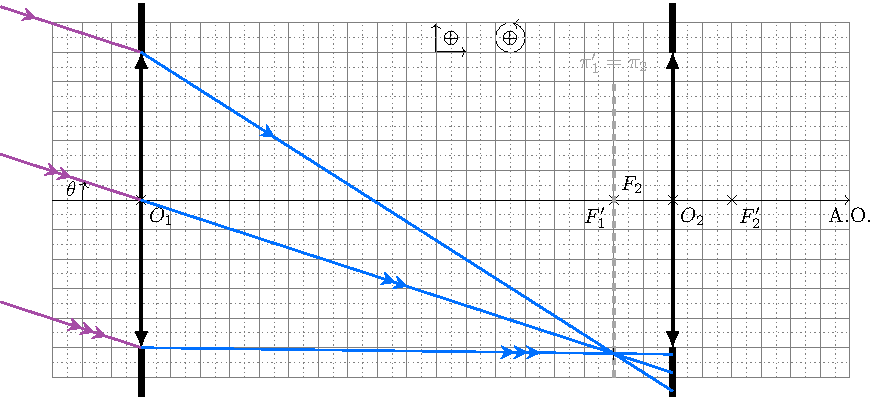
\includegraphics[width=\linewidth]{lunette3_corr}}
		\caption{}
		\label{fig:lunettes}
	\end{figure}

	\newpage
	\chapter*{Annexe~: problème 1}

	\begin{figure}[htbp]
		\centering
		\subcaptionbox{Cas où $n_g>n_{\rm liq}$\label{fig:gemme_c1}}
		{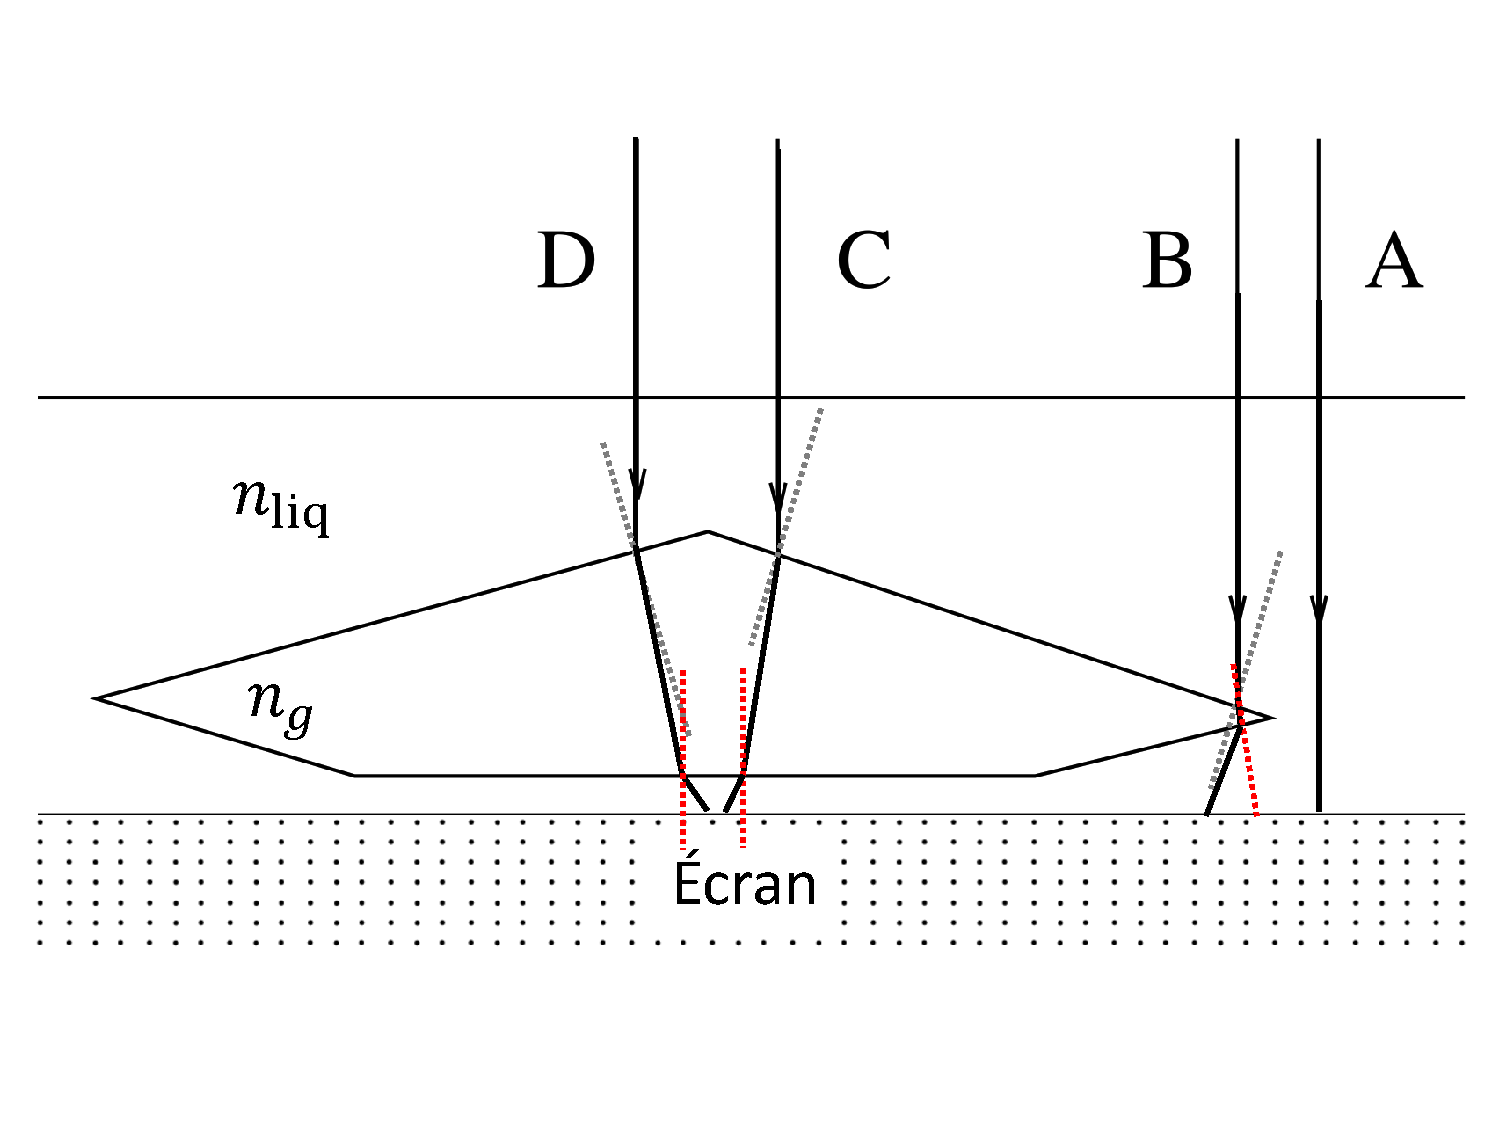
\includegraphics[width=.7\linewidth]{gemme_c1}}
		\subcaptionbox{Cas où $n_g<n_{\rm liq}$\label{fig:gemme_c2}}
		{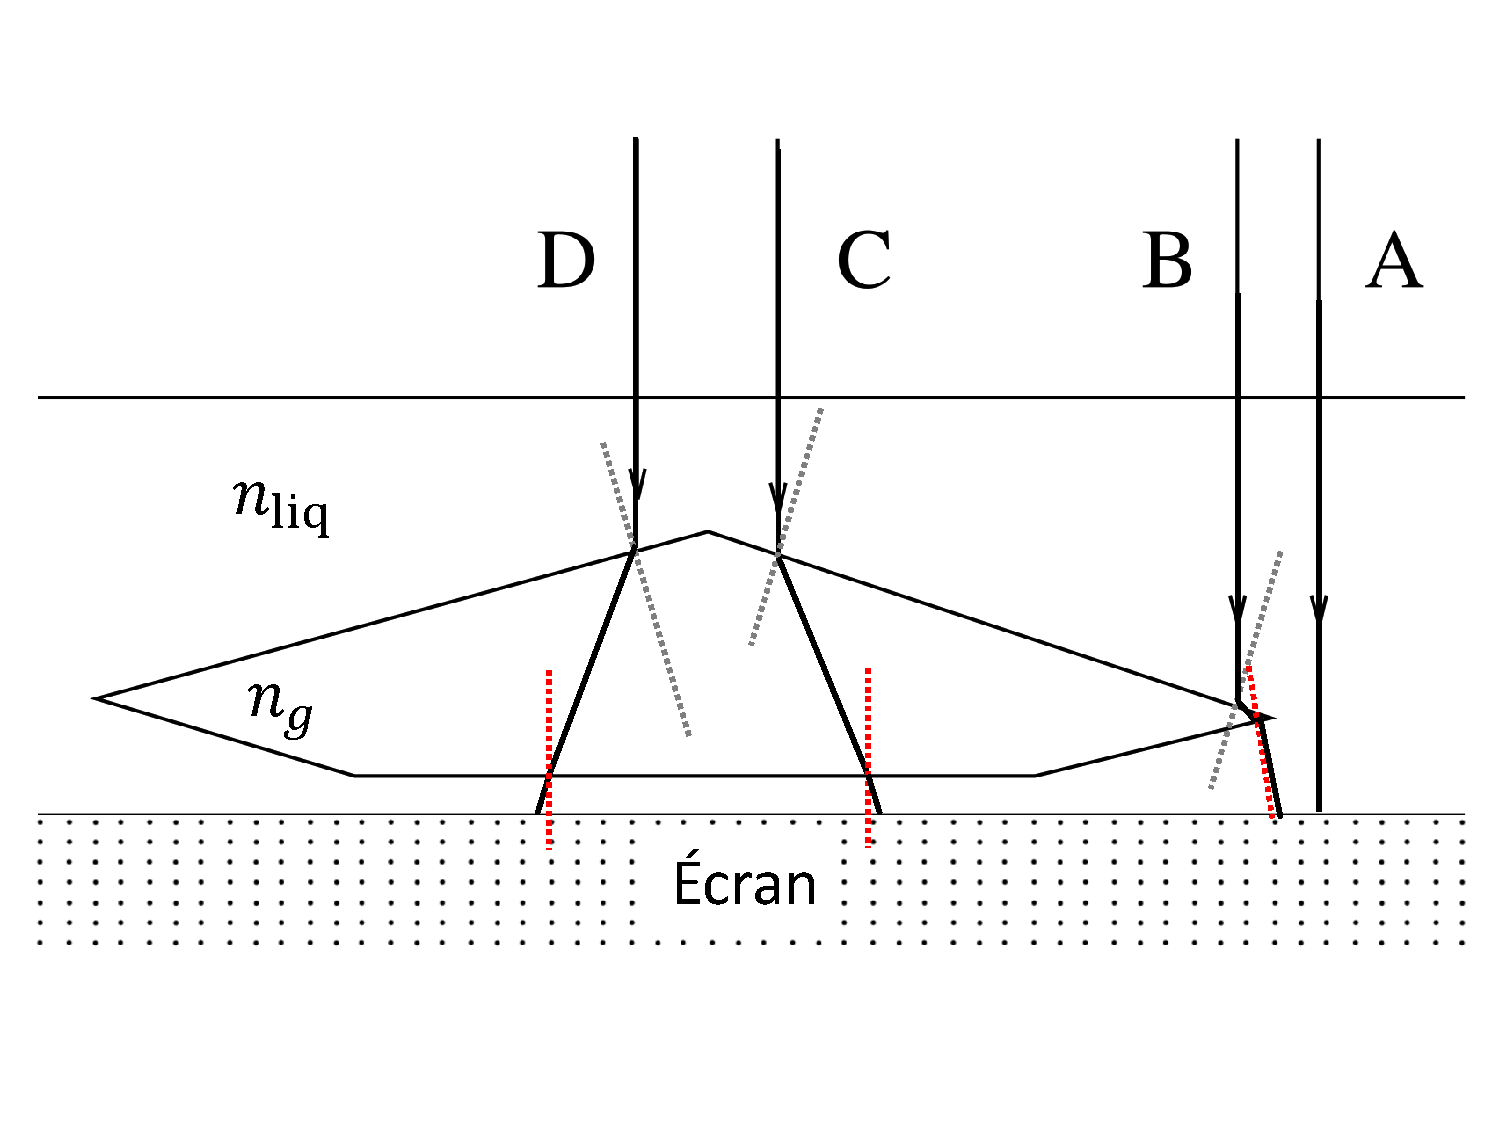
\includegraphics[width=.7\linewidth]{gemme_c2}}
		\caption{Annexe problème 2}
	\end{figure}

	\newpage
	\chapter*{Annexe~: problème 2}

	\begin{figure}[htbp!]
		\centering
		\subcaptionbox{Annexe question 2\label{fig:gob1}}
		[.75\linewidth]
		{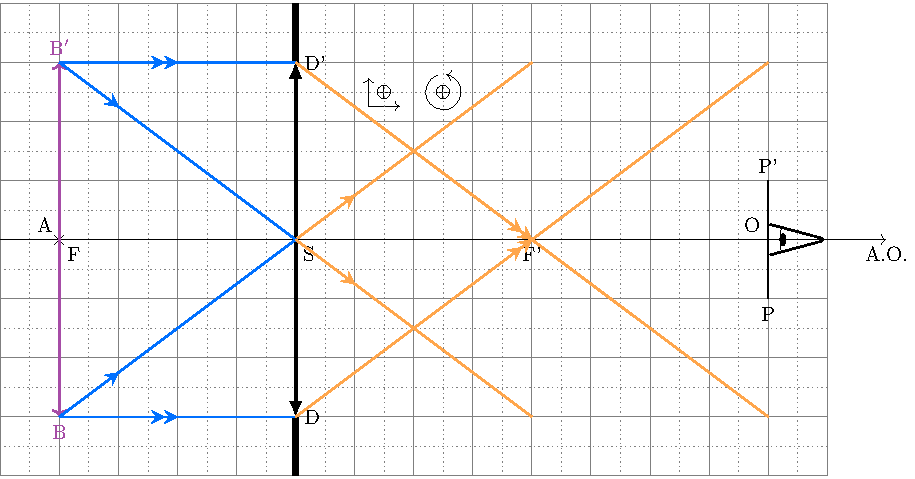
\includegraphics[width=\linewidth]{P1_1-corr}}
		\subcaptionbox{Annexe question 6\label{fig:gob2}}
		[.75\linewidth]
		{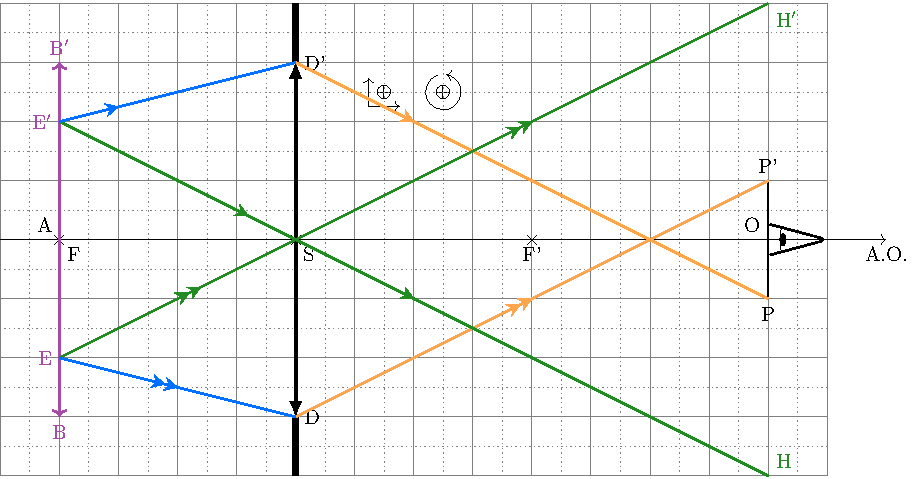
\includegraphics[width=\linewidth]{P1_2-corr}}
		\subcaptionbox{Annexe question 9\label{fig:gob3}}
		[.75\linewidth]
		{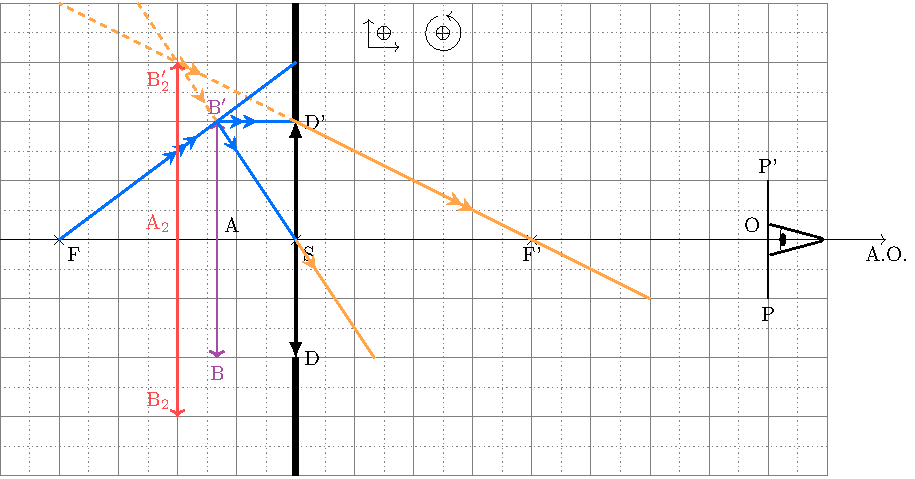
\includegraphics[width=\linewidth]{P1_3-corr}}
		\caption{}
		\label{fig:gob}
	\end{figure}
}
\vspace{-20pt}
\end{document}
